\documentclass{article}

% если нужно передать параметры в natbib, используйте, например:
\PassOptionsToPackage{numbers, compress}{natbib}
% до загрузки neurips_2026

% Авторам следует использовать один из следующих треков.
% До принятия на конференцию NeurIPS выберите один из вариантов ниже.
% 0. "default" для подачи
\usepackage{arxiv}
% параметр "default" эквивалентен параметру "main", который используется для Main Track с двойным слепым рецензированием.
% 1. параметр "main" используется для Main Track
%  \usepackage[main]{neurips_2026}
% 2. параметр "position" используется для Position Paper Track
%  \usepackage[position]{neurips_2026}
% 3. параметр "eandd" используется для Evaluations & Datasets Track
 % \usepackage[eandd]{neurips_2026}
 % если требуется подать деанонимизированную версию (не рекомендуется, но допустимо):
 %\usepackage[eandd, nonanonymous]{neurips_2026}
% 4. параметр "creativeai" используется для Creative AI Track
%  \usepackage[creativeai]{neurips_2026}
% 5. параметр "sglblindworkshop" используется для воркшопа с одинарным слепым рецензированием
 % \usepackage[sglblindworkshop]{neurips_2026}
% 6. параметр "dblblindworkshop" используется для воркшопа с двойным слепым рецензированием
%  \usepackage[dblblindworkshop]{neurips_2026}

% После принятия авторам следует добавить "final" после трека, чтобы скомпилировать camera-ready версию.
% 1. Main Track
 % \usepackage[main, final]{neurips_2026}
% 2. Position Paper Track
%  \usepackage[position, final]{neurips_2026}
% 3. Evaluations & Datasets Track
 % \usepackage[eandd, final]{neurips_2026}
% 4. Creative AI Track
%  \usepackage[creativeai, final]{neurips_2026}
% 5. Воркшоп с одинарным слепым рецензированием
%  \usepackage[sglblindworkshop, final]{neurips_2026}
% 6. Воркшоп с двойным слепым рецензированием
%  \usepackage[dblblindworkshop, final]{neurips_2026}
% Примечание. Для шаблона статьи воркшопа требуются и \title{}, и \workshoptitle{}: первая команда задает название статьи, показанное в заголовке, а вторая задает название воркшопа, отображаемое в сноске.
% Для воркшопов (5., 6.) авторам следует добавить название воркшопа; команда "\workshoptitle" используется для задания названия воркшопа.
% \workshoptitle{WORKSHOP TITLE}

% параметр "preprint" используется для arXiv или других препринтных подач
 % \usepackage[preprint]{neurips_2026}

% чтобы избежать загрузки пакета natbib, добавьте параметр nonatbib:
%    \usepackage[nonatbib]{neurips_2026}

\usepackage[utf8]{inputenc} % разрешить ввод utf-8
\usepackage[T2A,T1]{fontenc}    % поддержка кириллицы и латиницы
\usepackage[english,russian]{babel}
\usepackage{hyperref}       % гиперссылки
\usepackage{url}            % простая верстка URL
\usepackage{booktabs}       % таблицы профессионального качества
\usepackage{amsfonts}       % математические символы blackboard
\usepackage{nicefrac}       % компактные символы для 1/2 и т. п.
\usepackage{microtype}      % микротипографика
\usepackage{xcolor}         % цвета


%%%%%%%%%%%%%%%%%%%%%%%%%%%%%%%%%%%%%%%%%%%%%%%%%%%%%%%%%%%%%%%%%%%%%%%%

%%% Включите сюда любые пользовательские команды авторов.

\usepackage{algorithm}
\usepackage{algorithmic}
\usepackage{amsmath}
\usepackage{amssymb}
\usepackage{mathtools}
\mathtoolsset{showonlyrefs}
\usepackage{amsthm}

\usepackage{mathrsfs}
\usepackage{framed}
\usepackage{enumitem}
\usepackage{tcolorbox}

% \usepackage{cancel}

\newcommand{\ubar}[2]{\underbrace{#1}_{\mathclap{\text{#2}}}}
\newcommand{\obar}[2]{\overbrace{#1}^{\mathclap{\text{#2}}}}

\newcommand{\BibTeX}{\rm B\kern-.05em{\sc i\kern-.025em b}\kern-.08em\TeX}

\newcommand{\red}[1]{\textcolor{red}{#1}}
\newcommand{\as}[1]{\textcolor{magenta}{#1}}
% \newcommand{\asc}[1]{\textcolor{magenta}{ \small AS:~ #1}}


% \mathtoolsset{showonlyrefs=true}


%%%%%%%%%%%%%%%%%%%%%%%%%%%%%%%%
% ТЕОРЕМЫ
%%%%%%%%%%%%%%%%%%%%%%%%%%%%%%%%
\theoremstyle{plain}

\newtheorem{assumption}{Предположение}
\newtheorem{definition}{Определение}
\newtheorem{proposition}{Утверждение}
\newtheorem{remark}{Замечание}
\newtheorem{theorem}{Теорема}
\newtheorem{lemma}{Лемма}
\newtheorem{statement}{Утверждение}
\newtheorem{observation}{Наблюдение}
\newtheorem{example}{Пример}
\newtheorem{corollary}{Следствие}

% Определяем стиль для блока алгоритма
\newenvironment{algblock}{%
    \vspace{2pt}%
    \hspace*{-3mm}%
    \begin{minipage}{\linewidth}%
    % \vrule width 1.5pt \color{gray!50} \hspace*{2mm}%
    \hspace*{3mm}%
    \vrule width 1.5pt \hspace*{2mm}%
    \begin{minipage}{0.95\linewidth}%
}{%
    \end{minipage}%
    \end{minipage}%
    \vspace{2pt}%
}

\DeclareMathOperator*{\argmin}{argmin} %доп для argmin
\DeclareMathOperator*{\argmax}{argmax} %доп для argmax
\newcommand{\algname}[1]{{\textsf  #1}}
\newcommand{\mbR}{\mathbb R}
\newcommand{\mbE}{\mathbb E}
% \newcommand{\Edata}{\mbE_{(x, y) \sim D}}

\newcommand{\x}{\mathrm{x}}
\newcommand{\ERM}{\widehat L}
\newcommand{\Regret}[1]{\mathrm{Reg}_{\mathcal{P}}(#1)}
\newcommand{\ntrain}{n^t_k}
\newcommand{\LCB}{\texttt{LCB}}
\newcommand{\UCB}{\texttt{UCB}}
% \newcommand{\ft}[1]{l^t_{#1}\left(w_{#1}^{n_{#1}(t)}\right)}
\newcommand{\ft}[1]{l^t_{#1}\left(w_{#1}^{t}\right)}
\newcommand{\EDRB}{\texttt{ED}$^2$\texttt{RB}}

% нумерованные неравенства
\newcounter{ineqnumber}
\newcommand{\numleq}{\stepcounter{ineqnumber}\overset{(\arabic{ineqnumber})}{\leq}}
\newcommand{\numgeq}{\stepcounter{ineqnumber}\overset{(\arabic{ineqnumber})}{\geq}}
\newcommand{\numg}{\stepcounter{ineqnumber}\overset{(\arabic{ineqnumber})}{>}}
\newcommand{\numl}{\stepcounter{ineqnumber}\overset{(\arabic{ineqnumber})}{<}}
\newcommand{\numeq}{\stepcounter{ineqnumber}\overset{(\arabic{ineqnumber})}{=}}

% \newcommand{\red}[1]{\textcolor{red}{#1}}


\newcommand*{\comm}[1]{\begin{tcolorbox}[colback=blue!5!white,colframe=blue!75!black,title=Comment,fonttitle=\bfseries]#1\end{tcolorbox}}

% \newcommand{\as}[1]{\textcolor{magenta}{#1}}

\usepackage{mdframed}
\newmdenv[
    nobreak=true,    % предотвращает разрывы страниц внутри рамки
    % Можно дополнительно настроить внешний вид:
    % backgroundcolor=yellow!10,
    skipabove=\topskip,
    skipbelow=\topskip,
    linewidth=1pt
]{nframed}

% \mathtoolsset{showonlyrefs}
%%%%%%%%%%%%%%%%%%%%%%%%%%%%%%%%%%%%%%%%%%%%%%%%%%%%%%%%%%%%%%%%%%%%%%%%


% Примечание. Для шаблона статьи воркшопа требуются и \title{}, и \workshoptitle{}: первая команда задает название статьи, показанное в заголовке, а вторая задает название воркшопа, отображаемое в сноске.
\title{Управление самообучающимися экспертами при ограничениях бюджета на раунд}


% Макрос \author работает с любым числом авторов. Для разделения имен и адресов
% нескольких авторов используются две команды: \And и \AND.
%
% При использовании \And между авторами LaTeX сам определяет, где сделать
% перенос строки. Использование \AND принудительно вставляет перенос строки в этом месте.
% Поэтому, если LaTeX помещает имена 3 из 4 авторов на первую строку, а последнего —
% на вторую, попробуйте использовать \AND вместо \And перед именем третьего автора.


\author{%
  Ильгам Латыпов \\
  Московский Физико Технический Институт
  \AND
  Юрий Дорн
  % примеры дополнительных авторов
  % \And
  % Соавтор \\
  % Аффилиация \\
  % Адрес \\
  % \texttt{email} \\
  % \AND
  % Соавтор \\
  % Аффилиация \\
  % Адрес \\
  % \texttt{email} \\
  % \And
  % Соавтор \\
  % Аффилиация \\
  % Адрес \\
  % \texttt{email} \\
  % \And
  % Соавтор \\
  % Аффилиация \\
  % Адрес \\
  % \texttt{email} \\
}


\begin{document}


\maketitle


\begin{abstract}
        В данной работе рассматривается задача последовательного принятия решений при ограничениях на бюджет обучения. Такие постановки естественно возникают в приложениях, например при управлении портфелем алгоритмов бандитов или обучения с подкреплением (RL). Мы предлагаем новый алгоритм UCB-типа, M-LCB, предназначенный для управления набором из $K$ самообучающихся экспертов в стохастической среде с учетом ограниченного бюджета обучения на раунд $M$. На каждом раунде M-LCB выбирает одного эксперта для принятия решения и не более $M \le K$ экспертов для обучения. Для выбора M-LCB использует доверительные границы, построенные на основе ограниченных априорных знаний об экспертах (т. е. мягких предположений) и наблюдаемых обучающих потерь. Мы выводим anytime-оценки регрета для M-LCB, которые масштабируются с индивидуальными регретами экспертов. В частности, если каждый эксперт имеет регрет $\tilde O(T^\alpha)$ к раунду $T$, то M-LCB гарантирует общий регрет $\tilde O\left(\sqrt{KT/M} + (K/M)^{1-\alpha}T^\alpha\right)$ относительно лучшего эксперта в ретроспективе. Наконец, мы демонстрируем применимость M-LCB, задавая самообучающихся экспертов как (i) параметрические модели и (ii) бандитные алгоритмы.
\end{abstract}




\section{Введение}

Во многих приложениях необходимо динамически выбирать между несколькими моделями: рекомендательные системы могут запускать несколько предикторов параллельно, обновляя их по поступающей обратной связи от пользователей; финансовые платформы полагаются на переключение между торговыми стратегиями по мере изменения рыночных режимов; крупномасштабные онлайн-сервисы управляют портфелем контекстных бандитов или алгоритмов обучения с подкреплением. Цель таких сценариев состоит в динамическом выборе наиболее точной модели на каждом шаге при одновременном управлении ограниченным вычислительным бюджетом на обучение. Эта постановка относится к области последовательного принятия решений.

Классические алгоритмы многоруких бандитов (MAB) \cite{auer2002finite,bubeck2012regret,lattimore2020bandit}, применяемые к этой задаче, обычно предполагают статическое или состязательное распределение наград для каждой руки. Экспертные алгоритмы \cite{cesa2006prediction,hazan2016introduction} обычно требуют полной обратной связи и не учитывают скорость обучения экспертов. Ни один из подходов полностью не решает задачу управления несколькими одновременно обучающимися экспертами при бюджете обучения на раунд. Мы устраняем этот разрыв, предлагая процедуру, которая
объединяет предсказание с выборочным обучением, учитывая фиксированный вычислительный бюджет на раунд. В частности, вклад данной работы состоит в следующем:
\begin{itemize}
    \item \textbf{Новый мета-алгоритм UCB-типа (M-LCB)}: мы предлагаем M-LCB, новый мета-алгоритм типа Upper Confidence Bound (UCB). Он управляет пулом из $K$ самообучающихся экспертов в стохастической среде с учетом ограниченного бюджета обучения на раунд $M (M\le K)$.
    \item \textbf{Вычислительная эффективность}: мы предлагаем метод построения доверительных границ непосредственно по реализованным потерям. Он вычислительно эффективен и позволяет обойти необходимость дорогостоящей вспомогательной оптимизации.
    \item \textbf{Теоретический анализ}: мы оцениваем качество мета-алгоритма через индивидуальные скорости сходимости экспертов. Например, когда регреты экспертов имеют вид $\tilde O(n^\alpha)$, общий регрет масштабируется как $\tilde O(\sqrt{KT/M} + (K/M)^{1-\alpha}T^\alpha)$.
    \item \textbf{Расширение на multi-play бандиты:} мы показываем, что M-LCB расширяется на постановку multiple-play bandits и контролирует регрет подмножества top-$M$.
\end{itemize}


\subsection{Связанные работы}


\textbf{Самообучающиеся эксперты (руки).}
В работе \cite{dorn2025functional} вводятся самообучающиеся руки в постановке MAB: каждая рука является black-box параметрической функцией, генерирующей награду, а ее параметр обновляется после выбора этой руки. На каждом раунде обучающийся выбирает руку с помощью индекса UCB-типа, наблюдает награду, а затем обновляет соответствующий параметр.

\textbf{Выбор модели на мета-уровне.}
Работа \cite{foster2017parameter} вводит безпараметрическую агрегацию нескольких online learners в рамках полной информации. \textsc{CORRAL}~\cite{agarwal2017corralling} объединяет пул бандитных алгоритмов с помощью online-mirror descent (OMD) с логарифмическим барьером и importance-weighted обратной связью. Авторы выводят distribution-free гарантии в стохастических и состязательных постановках. В работе~\cite{cutkosky2021dynamic} предлагается мета-алгоритм динамической балансировки, основанный на известных выражениях скоростей регрета базовых обучающихся алгоритмов. В этой постановке регрет определяется относительно глобально оптимального действия, и за раунд обновляется только один обучающийся алгоритм. В отличие от этого, наша формулировка использует \emph{поэкспертные, prefix-hindsight} гарантии $U_k(T,\delta)$, определенные относительно локального оптимума каждого эксперта. Работа~\cite{dann2024data} устраняет необходимость в известных скоростях регрета за счет
онлайн-оценивания коэффициентов по каждому обучающемуся алгоритму,
получая высоковероятностные data-dependent гарантии выбора модели для стохастических бандитов (также при обновлении одного обучающегося алгоритма за раунд). Наиболее близкая к нашей постановка представлена в \cite{pacchiano2020model}.
В ней рассматривается выбор модели с использованием \emph{smoothing wrapper}.
Авторы показывают, что мета-алгоритм \algname{CORRAL} в сочетании с их wrapper достигает регрета
$\tilde O(\sqrt{TK} + K^\alpha T^{1 - \alpha} +K^{1 - \alpha}T^{\alpha}c(\delta))$, когда регрет базовых обучающихся алгоритмов удовлетворяет $O(T^{\alpha}c(\delta))$.
Подход динамической балансировки~\cite{cutkosky2021dynamic} дает сходную общую оценку
$\tilde O\left(\sqrt{KT} + K^{1-\alpha}T^{\alpha}c(\delta)\right)$. Эти оценки регрета совпадают со скоростью, получаемой нашим методом, когда за раунд можно обучать только одного эксперта. Наш алгоритм достигает того же порядка зависимости от $T$ и $\alpha$,
при этом дополнительно поддерживая одновременное обучение до $M$ адаптивных экспертов с доверительными интервалами, вычисляемыми непосредственно по реализованным потерям каждой руки.

\textbf{MAB с обновлениями нескольких рук.}
В этой постановке мета-процедура может обновлять или наблюдать несколько рук за раунд. Несколько работ рассматривают \emph{состязательный} случай.
\cite{seldin2014prediction} изучают предсказание с ограниченными советами (запрос не более $M$ рук).
Авторы получают оценку регрета $\tilde{O}\Big(\sqrt{\tfrac{K T \log K}{M}}\Big)$.
Она плавно интерполирует между случаем полной информации и бандитной постановкой.
В \cite{yun2018multi} представлена минимаксно-оптимальная оценка регрета $\tilde O\Big(\max\{\sqrt{KT/M},\,\sqrt{T\log K}\}\Big)$. В частности, она совпадает с нижними оценками из \cite{seldin2014prediction}. Однако эти работы предполагают необучающиеся руки (экспертов). В \emph{стохастическом} случае \cite{yun2018multi} рассматривает многорукого бандита с дополнительными наблюдениями: обучающийся выбирает одну руку и может наблюдать до $M$ дополнительных рук за раунд.
Они предлагают алгоритм \emph{KL-UCB-AO}, достигающий асимптотически оптимального \emph{логарифмического} регрета. Однако его область применимости ограничена из-за свойств правила выбора на основе Kullback-Leibler.

\textbf{Partial monitoring.}
В отличие от стандартного partial monitoring \cite{cesa2006prediction}, где потери оцениваются по сигналам, наша модель наблюдает реализованные потери выбранных экспертов. Ключевое отличие состоит в нашем Asm.~\ref{assumption:expert_regret}, которое предполагает известные скорости улучшения экспертов и позволяет использовать доверительные границы. Алгоритмы PM, удовлетворяющие этому предположению, тем не менее могут быть включены в нашу схему как базовые эксперты.

% {\color{red}
% \paragraph{Partial monitoring.}
% Эта структура обратной связи также связана с partial monitoring, где обучающийся наблюдает сигнал, а не весь вектор потерь; см., например, главу~6.4 в \cite{cesa2006prediction}. Отличие состоит в том, что алгоритмы partial monitoring обычно строят оценки потерь по сигналам, тогда как наша модель ограниченных советов получает реализованные потери выбранного подмножества экспертов. Более важно, что наш анализ опирается на предположение обучаемости в Asm.~\ref{assumption:expert_regret}: каждый эксперт улучшается со скоростью, контролируемой известной функцией. Эта структура отсутствует в стандартной формулировке partial monitoring и именно она позволяет строить доверительные границы для оптимальных значений экспертов. И наоборот, signal-based алгоритмы могут быть включены в нашу схему как базовые эксперты, если их гарантии обучения выражаются через Asm.~\ref{assumption:expert_regret}.
% }

\textbf{Multiple-play multi-armed bandits.}
В постановке \emph{multiple-play} (см. \cite{agrawal1990multi,uchiya2010algorithms})
мета-процедура выбирает $M$ рук за раунд и наблюдает semi-bandit обратную связь.
UCB-based алгоритмы для комбинаторных бандитов~\cite{kveton2015tight}
достигают регрета $\tilde O(\sqrt{KT/M})$ при стохастических наградах,
предоставляя базовую линию для анализа качества на уровне подмножеств. Эти результаты служат ориентиром для multiple-play MAB расширения \algname{M-LCB}. Таблица~\ref{tab:comparison_existing} сравнивает постановки задач.

\paragraph{Структура статьи.}
Раздел~\ref{sec:setup} формализует постановку.
Раздел~\ref{sec:algorithm} представляет алгоритм \algname{M-LCB}.
Раздел~\ref{sec:theoretical_analysis} содержит теоретический анализ, а Раздел~\ref{sec:proof} содержит доказательства. Раздел~\ref{sec:experiments} содержит эксперименты.

\begin{table*}[!h]
\centering
\small
\caption{
Предполагая $U_k(T,\delta)=O(T^{\alpha}c(\delta))$ при $\alpha \in [0,1]$ и полилогарифмической $c(\delta)$, мы сравниваем скорости регрета с точностью до логарифмических множителей ($\checkmark$ обозначает поддерживаемые свойства). Регрет следует Разделу~\ref{sec:multiple_play} для multiple-play bandits, специальным соглашениям для \cite{seldin2014prediction, yun2018multi} и Разделу~\ref{sec:global-regret} в остальных случаях.
\textbf{Наш алгоритм \algname{M-LCB} достигает оптимальных скоростей для обоих определений регрета.}}

\label{tab:comparison_existing}
\begin{tabular}{p{3cm}lp{1cm} p{1cm} p{5.0cm}}
\toprule
\textbf{Алгоритм / ссылка} & \textbf{Обучаемость} & \textbf{Multi-arm} & \textbf{Multiple-play} & \textbf{Скорость регрета (с точностью до log)} \\
\midrule
\textsc{CORRAL} + smoothing wrapper~\cite{pacchiano2020model}
& $\checkmark$ & $\times$ & $\times$ &
$\tilde O\!\left(\sqrt{KT} + K^{\alpha}T^{1-\alpha} + K^{1-\alpha}T^{\alpha}c(\delta)\right)$ \\[1pt]

\textsc{EXP3.P} + smoothing wrapper~\cite{pacchiano2020model}
& $\checkmark$ & $\times$ & $\times$ &
$\tilde O\!\left(\sqrt{KT} + K^{\frac{1-\alpha}{2-\alpha}}T^{\frac{1}{2-\alpha}}c(\delta)^{\frac{1}{2-\alpha}}\right)$ \\[1pt]

Dynamic Balancing~\cite{cutkosky2021dynamic}
& $\checkmark$ & $\times$ & $\times$ &
$\tilde O\!\left(\sqrt{KT} + K^{1-\alpha}T^{\alpha}c(\delta)\right)$ \\[1pt]

Prediction with Limited Advice~\cite{seldin2014prediction}
& $\times$ & $\checkmark$ & $\times$ &
$\tilde O\!\left(\sqrt{\tfrac{KT\log K}{M}}\right)$ \\[1pt]

H-INF~\cite{yun2018multi}
& $\times$ & $\checkmark$ & $\times$ &
$\tilde O\!\left(\max\{\sqrt{KT/M},\,\sqrt{T\log K}\}\right)$ \\[1pt]

UCB-based multiple-play bandits~\cite{kveton2015tight}
& $\times$ & $\times$ & $\checkmark$ &
$\tilde O\!\left(\sqrt{KT/M}\right)$ $\alpha = \frac{1}{2}$ \\[1pt]

\textbf{\algname{M-LCB} [данная работа]}
& $\checkmark$ & $\checkmark$ & $\checkmark$ &
$\tilde O\!\left(\sqrt{\tfrac{KT}{M}} + (K/M)^{1-\alpha}T^{\alpha}c(\delta)\right)$ \\
\bottomrule
\end{tabular}
\vspace{-1em}
\end{table*}

\section{Постановка задачи}
\vspace{-1em}
\label{sec:setup}
В этом разделе мы формализуем взаимодействие между мета-процедурой $\mathcal{P}$ и пулом обучаемых экспертов. Раздел~\ref{sec:losses} подробно описывает протокол взаимодействия. Раздел~\ref{sec:global-regret} определяет цель через кумулятивный регрет. Раздел~\ref{sec:arm-dynamics} характеризует динамику обучения экспертов, а Раздел~\ref{sec:examples} иллюстрирует нашу схему конкретными примерами в параметрическом обучении и выборе бандитов.

\vspace{-0.5em}
\subsection{Протокол процедуры}
\label{sec:losses}
\vspace{-0.75em}

Мы рассматриваем стохастическую online-задачу принятия решений с $K$ экспертами и бюджетом обучения на раунд $M$. Пусть $\mathbf{U}$ — пространство решений, а $\mathbf{E}$ — пространство исходов. Среда характеризуется функцией потерь $\ell: \mathbf{U} \times \mathbf{E} \to \mathbb{R}_+$. Каждый эксперт $k \in [K]$ действует на своем подпространстве $\mathbf{U}_k \subseteq \mathbf{U}$ и генерирует предсказание $u_k^t \in \mathbf{U}_k$ на раунде $t$.

Мета-процедура $\mathcal{P}$ управляет этим пулом экспертов. На каждом раунде $t$ $\mathcal{P}$ распределяет бюджет обучения на подмножество $S_t \subseteq [K]$ (где $|S_t| \le M$) и выбирает глобальное решение $u^t \in \mathbf{U}$, принимая совет выбранного эксперта. Затем среда раскрывает случайный исход $\xi^t$ со значениями в $\mathbf{E}$, и $\mathcal{P}$ несет глобальную потерю $\ell(u^t, \xi^t)$.

% Модель обратной связи является моделью ограниченных советов, а не стандартной single-play bandit обратной связью. Исход $\xi^t$ генерируется независимо от выбранного мета-процедурой эксперта, и после наблюдения $\xi^t$ потеря $\ell(u_k^t,\xi^t)$ вычислима для каждого обучаемого эксперта $k\in S_t$, который выдал предсказание. Таким образом, развернутое решение определяет потерю, понесенную $\mathcal{P}$, тогда как все эксперты в $S_t$ получают обратную связь и могут обновляться. Эта модель лежит между стандартной бандитной обратной связью, где наблюдается только развернутое решение, и полной информацией, где наблюдаются все $K$ экспертов.


Ключевым является то, что обучение экспертов отделено от непосредственного качества мета-процедуры $\mathcal{P}$. Эксперты обновляют свои внутренние параметры исключительно на основе собственной потери предсказания, $\ell(u_k^t, \xi^t)$, и только когда выбраны в обучающем множестве $S_t$. Это создает двойную роль для $\mathcal{P}$: она исследует, распределяя бюджет обучения (выбирая $S_t$ для улучшения определенных экспертов), и эксплуатирует, агрегируя совет выбранного эксперта для формирования итогового предсказания $u^t$ (см. Раздел~\ref{sec:algorithm}). Это взаимодействие отражает схему \emph{prediction with limited advice} \cite{seldin2014prediction}. Блок ниже суммирует протокол.
\begin{nframed}
\noindent
\textbf{Протокол: принятие решений с обучаемыми экспертами}\\[0.25em]
Для $t=1,2,\dots$:
\begin{enumerate}[leftmargin=2em]
    \item Выбрать $S_t\subseteq[K]$ с $|S_t|\le M$ и решение $u^t\in\mathbf U$.
    \item Наблюдать $\xi^t\sim D$ и понести потерю $\ell(u^t,\xi^t)$.
    \item Для каждого $k\in S_t$ вычислить $\ell(u_k^t,\xi^t)$ и обновить эксперта $k$.
\end{enumerate}
\end{nframed}

\subsection{Регрет}
\label{sec:global-regret}
Пусть $L(u) := \mathbb{E}_{\xi \sim \mathcal{D}}[\ell(u,\xi)]$ — ожидаемая потеря решения $u \in \mathbf{U}$. Оптимальная достижимая ожидаемая потеря $L_k^\star$ $k$-го эксперта и глобальный минимум $L^\star$ равны

\begin{equation}
\label{def:expeted_smallest_loss}
L_k^\star := \min_{u \in \mathbf{U}_k} L(u),
\qquad
L^\star := \min_{k \in [K]} L_k^\star.
\end{equation}
Цель $\mathcal{P}$ — минимизировать кумулятивный регрет относительно лучшего эксперта в пуле:
\begin{equation}
\label{eq:regret}
\mathrm{Reg}(T) := \sum_{t=1}^T \ell(u^t, \xi^t) - T \cdot L^\star.
\end{equation}
% Этот регрет обобщает классический стохастический MAB-регрет на функциональную постановку и согласуется со стандартной целью в стохастическом обучении.

Это определение следует стандартной формулировке регрета в литературе по стохастическим многоруким бандитам. Мы работаем при следующих стандартных предположениях о среде:
\begin{assumption}[Стохастические ограниченные потери]
\label{assumption:stochastic_losses}
На каждом раунде среда независимо генерирует $\xi^t \overset{\mathrm{iid}}{\sim} D$ из неизвестного распределения $D$ с носителем на $\mathbf{E}$.
Потери имеют вид $\ell:\mathbf{U}\times \mathbf{E}\to [0,1].$
\end{assumption}

\begin{remark}[Об ограниченности потерь]
Эта постановка рассматривает ограниченные потери. Однако ее можно расширить на неограниченный случай (например, субгауссовский или с тяжелыми хвостами). В частности, доказательства требуют другого выбора концентрационных неравенств. В этом случае гарантии регрета сохраняются с точностью до логарифмического члена.
\end{remark}



\subsection{Самообучающиеся эксперты}
\label{sec:arm-dynamics}
Каждый эксперт $k$ является online-алгоритмом обучения, который улучшается по мере выбора для обучения. Пусть $I_k(t) := \{\tau < t : k \in S_\tau\}$ обозначает множество раундов до времени $t$, на которых эксперт $k$ был выбран для обучения. Мы определяем $n_k^t := |I_k(t)|$ как общее число таких обновлений.
Мы характеризуем качество этих экспертов через \textit{anytime-оценку регрета}. Это гарантирует, что по мере обучения эксперта его решения $u_k^t$ сходятся к его оптимуму $L_k^\star$. Накопленная потеря и регрет равны
\begin{equation}
\label{def:experts_running_loss}
L_{k}(t) := \frac{1}{n^t_k} \sum_{\tau \in I_{k}(t)} \ell(u_k^\tau,\xi^\tau),
\quad
R_k(t) := n^t_k \left( L_{k}(t) - L_k^\star\right).
\end{equation}
\begin{assumption}[Anytime-оценка регрета эксперта]
\label{assumption:expert_regret}
Для любого $\delta\in(0,1)$ с вероятностью не менее $1-\delta$ для всех $t\ge 1$ выполнено $R_k(t) \le U_k(n_k^t,\delta),$
где $U_k(\cdot,\delta)$ не убывает.
\end{assumption}
Asm.~\ref{assumption:expert_regret} согласуется со стандартными метриками качества в многоруких бандитах. Далее мы показываем, что регрет в online-оптимизации ему удовлетворяет.


\subsection{Примеры}
\label{sec:examples}
\paragraph{Online-параметрическое обучение.} Пусть $\xi^t=(x_t,y_t) \overset{\mathrm{i.i.d.}}{\sim} D$, где распределение $D$ имеет носитель на $\mathbf{E} :=\mathcal X \times \mathcal Y$ и неизвестно. Мета-процедура $\mathcal P$ стремится предсказать $y_t$, наблюдая $x_t$, т. е. решает задачу обучения с учителем. Пространство решений — класс предикторов, $\mathbf{U} := \{u: \mathcal X \to \mathcal Y\}$.
$\mathcal P$ управляет пулом экспертов, являющихся алгоритмами Online Convex Optimization (OCO)~\cite{hazan2016introduction}.

Каждый эксперт $k \in [K]$ связан с пространством параметров $\mathbf W_k \subseteq \mathbb R^{d_k}$ и функцией предсказания $f_k: \mathbf W_k \times \mathcal X \to \mathcal Y$. Для любого $w \in \mathbf W_k$ отображение $f_k(w, \cdot)$ является предиктором в $\mathbf U$, поэтому пространство решений этого эксперта равно $\mathbf U_k := \{f_k(w, \cdot):\, w \in \mathbf W_k\} \subseteq \mathbf U.$
Оптимальный риск эксперта $k$ (см.~\eqref{def:expeted_smallest_loss}) превращается в $L_k^\star = \min_{w \in \mathbf W_k} \mathbb E_{(x, y) \sim D} [\ell(f_k(w, x), y)]$.

При выборе для обучения эксперт $k$ предсказывает $w^t_k \in \mathbf{W}_k$ и получает обратную связь $\ell(f_k(w^t_k, x_t), y_t)$. Например, если эксперт является оптимизатором Online Gradient Descent (OGD), предполагается, что потеря $\ell(f_k(w_k, \cdot), \cdot)$ выпукла и $G$-липшицева на $\mathbf{W}_k$. Эксперт обновляет параметры по правилу $w_k^{\tau+1} = \Pi_{\mathbf{W}_k} [w_k^{\tau} - \eta_{\tau} \nabla_{w} \ell(f_k(w_k^\tau, x_\tau), y_\tau)]$, где $\Pi_{\mathbf{W}_k}$ обозначает евклидову проекцию на $\mathbf{W}_k$, а $\eta_{\tau}$ — размер шага обучения. OCO-регрет характеризует качество таких экспертов,
\begin{equation}
\label{eq:regret_oco}
\overline{R}_k(t) := \sum_{\tau \in I_k(t)} \ell(u_k^\tau, \xi^\tau) - \min_{u \in \mathbf{U}_k} \sum_{\tau \in I_k(t)} \ell(u, \xi^\tau).
\end{equation}
Для OGD выполнено $\overline{R}_k(t) \leq O(GD_k\sqrt{n})$, где
$D_k := \mathrm{diam}(\mathbf{W}_k)$, а $t$ таково, что $|I_{k}(t)| = n$ \cite{hazan2016introduction}.

Лемма~\ref{lem:prefix_to_expected} связывает этот регрет с ожидаемым регретом (см. Asm.~\ref{assumption:expert_regret}) через концентрационную оценку. Следовательно, OGD-эксперты удовлетворяют предположению с
$U_k(n, \delta) = O\left(GD_k\sqrt{n} + \sqrt{n \log(n/\delta)}\right)$.



\paragraph{Алгоритмы многоруких бандитов.} Мотивированные AutoML и распределенной маршрутизацией, мы рассматриваем мета-процедуру $\mathcal{P}$, выбирающую наиболее эффективного среди $K$ самооптимизирующихся экспертов. Как и в Bandit Model Selection \cite{pacchiano2020model}, это сложно из-за нестационарной динамики обучения экспертов и высокой стоимости выборок. Каждый эксперт $k$ является стохастическим бандитом, выдающим решения $u_k^t$ из $m_k$-мерного симплекса $\Delta_k$ над конечным пространством действий $\mathcal{A}_k$, что делает глобальное пространство решений $\mathbf{U} = \bigcup_k \Delta_k$. Латентное состояние среды $\xi^t \sim D$ определяет потерю $\tilde{\ell}(a, \xi)$ для любого действия $a \in \mathcal{A}_k$ на раунде $t$. Потеря эксперта — это математическое ожидание $\ell(u_k, \xi) := \mathbb{E}_{a \sim u_k} [\tilde{\ell}(a, \xi)]$, с оптимальным риском $L_k^\star = \min_{a \in \mathcal{A}_k} \mathbb{E}_{\xi \sim D} [\tilde{\ell}(a, \xi)]$.

В нашей постановке limited-advice каждый обучаемый эксперт $k \in S_t$ предлагает $u_k^t$, семплирует действие $a_k^t \sim u_k^t$ и наблюдает бандитную обратную связь $\tilde{\ell}(a_k^t, \xi^t)$. Качество измеряется псевдо-регретом $R_k(t) = \sum_{\tau \in I_k(t)} \ell(u_k^\tau, \xi^\tau) - n_k L_k^\star$. Стандартные алгоритмы, такие как \algname{UCB}, удовлетворяют Asm.~\ref{assumption:expert_regret} с $U_k(n, \delta) = O(\sqrt{m_k n \log(n/\delta)})$. Поскольку мы наблюдаем семплированные потери, а не ожидания, реализация использует эмпирическое среднее $\tilde L_k(t)=\frac{1}{n_k^t}\sum_{\tau\in I_k(t)}\tilde{\ell}(a_k^\tau,\xi^\tau)$. Добавление концентрационного члена для семплирования к $U_k$ обеспечивает корректные anytime высоковероятностные границы для работы алгоритма; подробный вывод см. в Приложении \ref{sup:bandit_application}.

\section{Алгоритм \algname{M-LCB}}
\label{sec:algorithm}
% Мы следуем оптимистическому принципу для обучения и консервативному принципу для deployment. На каждом раунде он распределяет бюджет обучения на экспертов, определенных как потенциально оптимальные с помощью нижних доверительных границ (LCB). Поскольку потери минимизируются, низкая LCB указывает, что эксперт может иметь малую оптимальную потерю $L_k^\star$ и потому заслуживает обучения. Однако среди обучаемых экспертов развертываемый советчик выбирается с помощью верхних доверительных границ (UCB): минимизация UCB контролирует потерю текущего раунда. Использование LCB для обеих ролей чрезмерно эксплуатировало бы неопределенных экспертов, текущая потеря которых может оставаться большой.

% Для реализации этой стратегии мы строим для каждого эксперта $k$ $\LCB_k(t, \cdot)$ и $\UCB_k(t, \cdot)$---нижнюю и верхнюю доверительные границы неизвестной оптимальной потери $L_k^\star$ (см.~\eqref{def:expeted_smallest_loss}), эффективно вычисляемые по накопленной потере $L_k(t)$ (см.~\eqref{def:experts_running_loss}).
Мы балансируем оптимистическое обучение с консервативным deployment: распределяем бюджет обучения на потенциально оптимальных экспертов с наименьшими нижними доверительными границами ($LCB_k$), одновременно выбирая развертываемого советчика по наименьшим верхним доверительным границам ($UCB_k$), чтобы минимизировать немедленную потерю. Это предотвращает чрезмерную эксплуатацию неопределенных экспертов.


\begin{definition}[UCB и LCB]
\label{def:ucb_lcb}
Зафиксируем $k\in[K]$ и положим
\begin{align*}
\LCB_k(t,\delta)
:= L_{k}(t)- \tfrac{U_k\left(n^t_k,\delta_{\mathrm{arm}}\right)}{n^t_k}, \quad
\UCB_k(t,\delta)
:= L_{k}(t) + H(n^t_k,\delta_{n^t_k}),
\end{align*}
где $\delta_{\mathrm{arm}} = \tfrac{\delta}{2K}$,  $\delta_n = \tfrac{\delta}{3.5Kn^2}$ и $H(n,\delta) = \sqrt{\tfrac{2\log(1/\delta)}{n}}$,
при этом $U_k(\cdot)$ — оценка регрета из Asm.~\ref{assumption:expert_regret}, а $L_k(t)$ — накопленная потеря, определенная в \eqref{def:experts_running_loss}.
\end{definition}


На раунде $t$ мы вычисляем $\LCB_k(t,\delta)$ и $\UCB_k(t,\delta)$ для каждого эксперта $k$. Затем определяем обучающее подмножество $S_t$ и советчика $i_t$ по следующим правилам:
\begin{align*}
S_t &:= \arg\min_{\substack{S\subseteq[K]\\ |S|=M}} \sum_{k\in S}\LCB_k(t,\delta), ~~
i_t = \arg\min_{k\in S_t}\UCB_k(t,\delta).
\end{align*}

Чтобы преодолеть отсутствие поточечной сходимости в стохастических алгоритмах \cite{cesa2006prediction, shalev2012online, pacchiano2020model}, мы используем smoothing wrappers \cite{orabona2019modern, pacchiano2020model} для устойчивого построения решения $u^t$ эксперта $i_t$, обеспечивая выполнение Asm.~\ref{assumption:wrapper} для $\mathcal{P}$. В отличие от состязательной агрегации экспертов (даже при $M=K$), наши доверительные границы оценивают оптимальные значения, напрямую используя структурные гарантии обучаемости базовых экспертов.

% Ключевая идея алгоритма состоит в устойчивом построении решения $u^t$, принимаемого экспертом $i_t$ на раунде $t$. В частности, стохастические алгоритмы (например, градиентные методы, бандитные алгоритмы) часто гарантируют сходимость только в среднем или по распределению, но не поточечно по последней итерации; см. \cite{cesa2006prediction, shalev2012online, pacchiano2020model}. Вдохновленные online-to-batch conversion \cite{orabona2019modern, pacchiano2020model}, мы вводим smoothing wrappers. Поэтому решение, принимаемое $\mathcal{P}$, основано на истории обучения выбранного эксперта $i_t$ и удовлетворяет Asm.~\ref{assumption:wrapper}. Эта схема не является агрегацией состязательных экспертов даже при $M=K$: доверительные границы используют структурные гарантии обучаемости базовых экспертов для оценки их оптимальных значений.

\begin{assumption}[Smoothing wrapper]
\label{assumption:wrapper}
Smoothing wrapper — возможно рандомизированное отображение $\upsilon$, которое принимает конечную последовательность решений
$H=\{u^\tau:\tau\in Z\}\subseteq \mathbf U$ с $|Z|\ge 1$ и возвращает решение $u=\upsilon(H)\in\mathbf U$
такое, что
\begin{equation*}
\mathbb E_{u\sim v(H)}\bigl[L(u)\mid H\bigr]\ \le\ \frac{1}{|Z|}\sum_{\tau\in Z} L(u^\tau),
\qquad
L(u):=\mathbb E_{\xi\sim D}[\ell(u,\xi)].
\end{equation*}
\end{assumption}

\begin{example}
\label{example:wrapper}
Предположим, что $\mathbf U$ выпукло и $\ell(\cdot,\xi)$ выпукла по $u$ для всех $\xi$. Естественный выбор — среднее $u = \frac{1}{|Z|}\sum_{\tau\in Z} u^\tau,$
которое удовлетворяет Asm.~\ref{assumption:wrapper} по неравенству Йенсена. Рандомизированная форма Asm.~\ref{assumption:wrapper} также покрывает невыпуклые пространства решений: можно равномерно семплировать $u$ из истории $\{u^\tau:\tau\in Z\}$ \cite{pacchiano2020model}; в этом случае требуемое неравенство выполняется в условном математическом ожидании без требования выпуклости.
\end{example}

Alg.~\ref{algorithm:M_LCB} описывает процедуру. Инициализация каждого эксперта один раз перед основным циклом обеспечивает корректно определенные доверительные границы и стоит не более $K$ обновлений, не влияя на асимптотический регрет. Шаг \textit{Update} обрабатывает как внутреннее обучение, так и учетные переменные (например, счетчики, накопленную потерю).

% Alg.~\ref{algorithm:M_LCB} подробно описывает процедуру. Перед основным циклом каждый эксперт инициализируется один раз, чтобы все доверительные границы были корректно определены; это стоит не более $K$ дополнительных обновлений и не влияет на асимптотические скорости регрета.
% Шаг \textit{Update} для эксперта включает его внутреннее обновление обучения, а также обновление соответствующих учетных переменных (счетчиков, накопленной потери и т. д.).

\begin{algorithm}[ht!]
\caption{\algname{M-LCB}}
\label{algorithm:M_LCB}
\begin{algorithmic}[1]
\STATE \textbf{Вход:} эксперты $\{\mathbf{U}_k\}_{k=1}^K$, бюджет на раунд $M$, параметр доверия $\delta$, smoothing wrapper $\upsilon$ (см. Предположение \ref{assumption:wrapper}).

\STATE \textbf{Выход:} (i) последовательность советов $\{u^t\}_{t=1}^T$; (ii) эксперты, обучаемые на каждом раунде $\{S_t\}_{t=1}^T$

\STATE Инициализировать каждого эксперта с $\delta_{\mathrm{arm}} = \delta/(2K)$ (см. Def.~\ref{def:ucb_lcb})
\STATE Выполнить warm-start каждого эксперта один раз, чтобы $n_k^t\ge 1$ для всех $k$ до применения основного правила выбора.
\FOR{$t=1,2,\dots,T$}
    \FOR{каждого $k \in [K]$}
        \STATE Вычислить $\LCB_k(t,\delta), \UCB_k(t,\delta)$
    \ENDFOR
    \STATE $S_t \gets \arg\min_{S\subseteq[K],|S|=M}\sum_{k\in S}\LCB_k(t,\delta)$
    \STATE $i_t \gets \arg\min_{k\in S_t}\UCB_k(t,\delta)$
    \STATE $u^t \gets \upsilon(\{u_{i_t}^\tau: \tau \in I_{i_t}(t)\})$ \hfill // сглаживание по $i_t$
    \STATE Сыграть $u^t$, понести $\ell(u^t,\xi^t)$
    \FOR{каждого $k \in S_t$}
        \STATE Наблюдать $\ell(u_k^t, \xi^t)$.
        \STATE Обновить эксперта $k$.
    \ENDFOR
\ENDFOR
\end{algorithmic}
\end{algorithm}



\section{Оценки регрета}
\label{sec:theoretical_analysis}
Пусть \emph{концентрационное событие $\mathcal{E}_{\delta}$} гарантирует, что все доверительные границы выполняются одновременно для каждого эксперта и каждого шага времени (подробности см. в Лемме~\ref{prop:anytime-ci-clear}). Сначала мы устанавливаем высоковероятностные оценки псевдо-регрета и реализованного регрета.
\begin{lemma}[Оценки регрета]
\label{lem:regret_bounds}
Пусть псевдо-регрет равен
\begin{equation}
% \label{eq:regret}
\widetilde{\mathrm{Reg}}(T)
:= \mathbb E_{\upsilon}\left[\sum_{t=1}^T L(u^t)\right]  - T \cdot L^\star,
\end{equation}
где математическое ожидание берется по возможной рандомизации smoothing wrapper.
При $L(\cdot) := \mathbb{E}_{\xi \sim \mathcal{D}}[\ell(\cdot,\xi)]$ зафиксируем $\delta \in (0,1)$ и предположим, что выполнены Предположения~\ref{assumption:stochastic_losses}-\ref{assumption:wrapper}.
Тогда для псевдо-регрета Alg.~\ref{algorithm:M_LCB} на концентрационном событии $\mathcal{E}_{\delta}$ для всех $T\ge 1$ выполнено $\widetilde{\mathrm{Reg}}(T) \le \mathbb E_{\upsilon}[\Delta(T)]$, где
\begin{align}
\label{eq:bound_bound_bound}
    \Delta(T) :=
     \sum_{\tau \in I_{k^{\star}}(T)} \bigl[\UCB_{k^\star}(\tau, \delta)-\LCB_{k^\star}(\tau, \delta)\bigr]
    + \frac{1}{M}\sum_{k=1}^K \sum_{{\tau \in I_{k}(T)}} \bigl[\UCB_k(\tau, \delta)-\LCB_k(\tau, \delta)\bigr],
\end{align}

    где $k^\star$ — индекс лучшего эксперта.
Более того, с вероятностью не менее $1-2\delta$ для всех $T\ge 1$ выполнено $\mathrm{Reg}(T) \le \mathbb E_{\upsilon}[\Delta(T)] + O(\sqrt{T}).$
\end{lemma}

Мы конкретизируем этот результат для случая, когда регреты экспертов имеют вид $\tilde O(n^\alpha)$.

\begin{theorem}[Скорости сходимости]
\label{thm:gen-rate}
Пусть $\alpha, \delta \in (0, 1)$, и каждый эксперт $k$ удовлетворяет Asm.~\ref{assumption:expert_regret}
с $U_k(t,\delta) =O\big(t^{\alpha}c(\delta)\big)$.
Тогда с вероятностью не менее $1 - \delta$ регрет Alg.~\ref{algorithm:M_LCB} ограничен для всех $T\ge1$ следующим образом:
\begin{equation*}
\mathrm{Reg}(T)
= O\left(\sqrt{\frac{K T}{M}\log(\frac{KT}{\delta})} + \Bigl(\tfrac{K}{M}\Bigr)^{1-\alpha} T^{\alpha} c(\delta)\right).
\end{equation*}
\end{theorem}
Мы также получаем нижние оценки.
\begin{definition}[Стохастические задачи с нижней оценкой $\alpha$–регрета]
\label{def:alpha-class}
Пусть $\alpha \in [0,1]$.
Семейство $\mathcal{F}_\alpha$ стохастических online-задач обучения допускает \emph{нижнюю оценку $\alpha$–регрета},
если для любого алгоритма обучения $\mathscr{A}$ и любого $T \ge 1$ выполнено $\sup_{f \in \mathcal{F}_\alpha}
\mathbb{E}\bigl[R_{\mathscr{A}}(T)\bigr]
\ge
c\,T^{\alpha},$
для некоторой константы $c > 0$, не зависящей от\, $T$ и $\mathscr{A}$.
\end{definition}

\begin{theorem}[Нижняя оценка]
\label{thm:mt-alpha}
Рассмотрим $K$ экспертов, горизонт $T$ и бюджет на раунд $M$. Зафиксируем $\alpha\in[0,1]$. Существует класс $\mathcal F_\alpha$, удовлетворяющий Def.~\ref{def:alpha-class}, такой, что если каждый
эксперт $k \in [K]$ решает задачу $f_k \in \mathcal F_\alpha$, то при достаточно малом $\sqrt{\frac{K\log K}{MT}}$ и для любого алгоритма $\mathscr{A}_k$ и мета-процедуры $\mathcal{P}$
\begin{equation}
\label{eq:mt-alpha-internal_appendix}
\sup_{f_{k} \in \mathcal{F}_{\alpha},\,k \in [K]} \mathbb{E}\,\mathrm{Reg}(T) \ge c_1\,\sqrt{\frac{K\,T}{M}}
\;+\; c_2\,T^\alpha \left(\frac{K}{M} \right)^{1-\alpha},
\end{equation}
где $c_1,c_2>0$ — абсолютные константы.
\end{theorem}
Это устанавливает фундаментальную нижнюю границу для управления обучаемыми экспертами при бюджете: исследование ($\sqrt{KT/M}$) доминирует при $\alpha<1/2$, тогда как обучение экспертов ($T^\alpha (K/M)^{1-\alpha}$) доминирует при $\alpha\ge 1/2$. Для ограниченных потерь наш алгоритм \algname{M-LCB} совпадает с этой границей с точностью до логарифмических множителей (доказательство Теоремы~\ref{thm:mt-alpha} в Приложении).

% Этот результат устанавливает фундаментальный предел качества для управления несколькими обучаемыми экспертами при бюджете на раунд. Для $\alpha<1/2$ член исследования $\sqrt{KT/M}$ доминирует в нижней оценке; для $\alpha\ge 1/2$ член обучения экспертов $T^\alpha (K/M)^{1-\alpha}$ является доминирующим вкладом.
% Мы предлагаем алгоритм \algname{M-LCB}, совпадающий с нижней оценкой с точностью до логарифмического множителя в случае ограниченной потери.
% Доказательство Теоремы~\ref{thm:mt-alpha} находится в Приложении.

\noindent
\textbf{Идея доказательства.}
Мы используем MAB с тяжелыми хвостами \cite{bubeck2013bandits} для построения $\mathcal{F}_{\alpha}$. Ключевые ингредиенты взяты из \cite{bubeck2010bandits, seldin2014prediction}. Члены в оценке возникают соответственно из сложности исследования и сложности обучения экспертов.





\subsection{Связь с Multiple-Play Bandits}
\label{sec:multiple_play}
\algname{M-LCB} расширяется на постановку multiple-play bandit \cite{agrawal1990multi, uchiya2010algorithms} путем deployment всех $M$ экспертов из $S_t$ и учета их средней потери. Качество оценивается относительно оптимального подмножества из $M$ экспертов; примечательно, что в этой постановке UCB-based алгоритмы \cite{kveton2015tight} достигают скоростей сходимости $\tilde O(\sqrt{KT/M})$ при фиксированных стохастических наградах.

% Наша постановка обобщает эту идею: вместо статических стохастических рук каждый выбранный элемент является самообучающимся экспертом, качество которого меняется со временем.
% Следующее утверждение формализует эту связь, показывая, что среднее качество подмножеств, обучаемых нашим алгоритмом,
% приближается к качеству лучших $M$ экспертов.

\begin{lemma}[Регрет top-$M$ экспертов]
\label{prop:m_mean_regret}
Зафиксируем $\delta \in (0,1)$
и предположим, что условия Леммы~\ref{lem:regret_bounds} выполнены.
Пусть $\overline{L}^\star = \min_{S\subseteq[K],\,|S|=M}\frac{1}{M}\sum_{k\in S}L_k^\star$ — средняя оптимальная потеря среди $M$ лучших экспертов. Пусть $\mathrm{Reg}_M(T) := \sum_{t=1}^{T}
\left[\frac{1}{M}\sum_{k \in S_t} L^\star_k - \overline{L}^\star \right].$ Следующая оценка выполняется с вероятностью не менее $1-\delta$: $$     \mathrm{Reg}_M(T) \le \frac{1}{M}\sum_{k=1}^K \sum_{{\tau \in I_{k}(T)}} \bigl[\UCB_k(\tau, \delta)-\LCB_k(\tau, \delta)\bigr].$$
\end{lemma}

Доказательство представлено в Приложении \ref{proof:m_mean_regret}. Это немедленно дает скорость сходимости для среднего top-$M$ регрета.

\begin{theorem}[Скорость сходимости для среднего top-$M$ регрета]
\label{thm:gen-rate-topM}
Пусть $\alpha\in(0,1]$, $\delta\in(0,1)$. Пусть каждый эксперт $k$ удовлетворяет
Asm.~\ref{assumption:expert_regret} с $U_k(t,\delta)=O\big(t^{\alpha}c(\delta)\big)$.
Запустим Alg.~\ref{algorithm:M_LCB} с доверительными границами из
Def.~\ref{def:ucb_lcb}. Тогда с вероятностью не менее $1 - \delta$ средний регрет выбранных рук $R(T)$ (см. Prop.~\ref{prop:m_mean_regret}) для всех $T\ge 1$ равен
\begin{equation*}
\mathrm{Reg}_M(T)= O\left(
\sqrt{\frac{KT}{M}\log\frac{KT}{\delta}} +
\Bigl(\frac{K}{M}\Bigr)^{1-\alpha} T^{\alpha} c(\delta)
\right).
\end{equation*}
\end{theorem}

Доказательство аналогично доказательству Теоремы \ref{thm:gen-rate}.

% \begin{table*}[t]
% \centering
% \small
% \caption{
% Сравнение со связанными результатами.
% Мы предполагаем, что $U_k(T,\delta)=O(T^{\alpha}c(\delta))$ при $\alpha \in [0,1]$,
% где $c(\delta)$ обычно полилогарифмична. Для \emph{multiple-play bandits} регрет как в Разделе~\ref{sec:multiple_play}.
% Для \cite{seldin2014prediction, yun2018multi} регрет определяется как для экспертных алгоритмов (см. статьи).
% Для остальных методов регрет как в Разделе~\ref{sec:global-regret}.
% Все скорости указаны с точностью до логарифмических множителей.
% Символ $\checkmark$ отмечает поддерживаемые свойства.
% \textbf{Наш алгоритм \algname{M-LCB} достигает оптимальных скоростей для обоих определений регрета.}}
% \label{tab:comparison_existing}
% \begin{tabular}{p{4.8cm}ccc p{5.5cm}}
% \toprule
% \textbf{Алгоритм / ссылка} & \textbf{Обучаемость} & \textbf{Multi-arm} & \textbf{Multiple-play} & \textbf{Скорость регрета (с точностью до log)} \\
% \midrule
% \textsc{CORRAL} + smoothing wrapper~\cite{pacchiano2020model}
% & $\checkmark$ & $\times$ & $\times$ &
% $\tilde O\!\left(\sqrt{KT} + K^{\alpha}T^{1-\alpha} + K^{1-\alpha}T^{\alpha}c(\delta)\right)$ \\[1pt]

% \textsc{EXP3.P} + smoothing wrapper~\cite{pacchiano2020model}
% & $\checkmark$ & $\times$ & $\times$ &
% $\tilde O\!\left(\sqrt{KT} + K^{\frac{1-\alpha}{2-\alpha}}T^{\frac{1}{2-\alpha}}c(\delta)^{\frac{1}{2-\alpha}}\right)$ \\[1pt]

% Dynamic Balancing~\cite{cutkosky2021dynamic}
% & $\checkmark$ & $\times$ & $\times$ &
% $\tilde O\!\left(\sqrt{KT} + K^{1-\alpha}T^{\alpha}c(\delta)\right)$ \\[1pt]

% Prediction with Limited Advice~\cite{seldin2014prediction}
% & $\times$ & $\checkmark$ & $\times$ &
% $\tilde O\!\left(\sqrt{\tfrac{KT\log K}{M}}\right)$ \\[1pt]

% H-INF~\cite{yun2018multi}
% & $\times$ & $\checkmark$ & $\times$ &
% $\tilde O\!\left(\max\{\sqrt{KT/M},\,\sqrt{T\log K}\}\right)$ \\[1pt]

% UCB-based multiple-play bandits~\cite{kveton2015tight}
% & $\times$ & $\times$ & $\checkmark$ &
% $\tilde O\!\left(\sqrt{KT/M}\right)$ $\alpha = \frac{1}{2}$ \\[1pt]

% \textbf{\algname{M-LCB} [данная работа]}
% & $\checkmark$ & $\checkmark$ & $\checkmark$ &
% $\tilde O\!\left(\sqrt{\tfrac{KT}{M}} + (K/M)^{1-\alpha}T^{\alpha}c(\delta)\right)$ \\
% \bottomrule
% \end{tabular}
% \end{table*}


\begin{remark}[О константах]
\label{rem:beta_dependence}
Если константы $\beta_k$ во внутренних оценках, $U_k(t,\delta)=O(\beta_k\,t^{\alpha}c(\delta))$, существенны
(например, зависят от размерности или липшицевой константы задачи),
то оценка регрета уточняется до
\begin{equation}
O\left(
\sqrt{\tfrac{KT}{M}\log(\tfrac{KT}{\delta})}
+ T^{\alpha} c(\delta) \left[ \beta_{k^\star} +
\Bigl(\tfrac{1}{M}\sum_{k=1}^K \beta_k^{\frac{1}{1-\alpha}}\Bigr)^{1-\alpha} \right] \right).
\end{equation}
что дает более точную характеристику зависимости от индивидуальных сложностей экспертов.
.
\end{remark}


\subsection{Сравнение с существующими результатами}
\label{sec:comparison}

Таблица~\ref{tab:comparison_existing} перечисляет мета-алгоритмы, используемые для выбора модели и бюджетированного multi-arm обучения.
Она показывает, поддерживает ли каждый метод \emph{обучаемых экспертов}, \emph{multi-arm обновления} и гарантии на \emph{multi-play регрет} (среднюю потерю выбранных подмножеств).

Алгоритмы выбора модели, такие как \cite{pacchiano2020model,cutkosky2021dynamic}, достигают оптимальных по порядку скоростей по $T$ и $K$ для обновлений одной руки,
предполагая известные или оцененные границы регрета экспертов $U_k(T,\delta)$. Однако они
не учитывают бюджеты обучения на раунд и качество на уровне подмножеств.
Методы multi-play bandit \cite{seldin2014prediction,yun2018multi,kveton2015tight}
обрабатывают бюджетированные обновления, но не обучают руки.

\textbf{\algname{M-LCB}} объединяет эти задачи:
он управляет \emph{обучаемыми экспертами} посредством \emph{нескольких обновлений экспертов за раунд}. Более того, он расширяется на постановку \emph{multi-play} и достигает той же оптимальной по порядку скорости для соответствующих регретов.

Дополнительные примеры применимых задач и базовых алгоритмов см. в Приложении~\ref{sup:applications}.


\section{Доказательства}
\label{sec:proof}
\setcounter{ineqnumber}{0}
\begin{proof}[Доказательство Леммы~\ref{lem:regret_bounds}]
\label{proof:regret_bound}
\textbf{Оценка псевдо-регрета}. $S_t$ и $i_t$ обозначают соответственно обучающее подмножество и руку предсказания, выбранные на раунде $t$ алгоритмом Alg.~\ref{algorithm:M_LCB}.
Пусть $k^\star \in \arg\min_{k\in[K]} L_k^\star$ — индекс лучшей руки по ожидаемой потере.

Алгоритм использует доверительные границы из Prop.~\ref{prop:anytime-ci-clear}, поэтому $\mathcal{E}_\delta$ ~\eqref{eq:conf_intervals} выполняется с вероятностью не менее $1-\delta$. Далее мы условимся на $\mathcal{E}_{\delta}$ и докажем оценки регрета на этом событии. При событии $\mathcal{E}_\delta$ безопасный совет в момент $t$ имеет вид $u^t = \upsilon(\{u_{i_t}^\tau: \tau \in I_{i_t}(t)\})$. По Asm.~\ref{assumption:wrapper} и определению $\mathcal{E}_\delta$ его условная ожидаемая потеря ограничена $\UCB_{i_t}(t,\delta)$. Следовательно,
\begin{equation}\label{eq:best-reg-start}
\widetilde{\mathrm{Reg}}(T) = \mathbb E_{\upsilon}\left[\sum_{t=1}^{T}\bigl[L(u^t) - L^\star\bigr]\right]
\le \mathbb E_{\upsilon}\left[\sum_{t=1}^{T}\bigl[\UCB_{i_t}(t, \delta) - L^\star\bigr]\right],
\end{equation}
где внешнее математическое ожидание опущено, поскольку все последующие неравенства выполняются поточечно для каждой реализованной последовательности выборов wrapper. Разбивая сумму в зависимости от того, обучается ли $k^\star$ в момент $t$, получаем
\begin{equation}
\overline{\mathrm{Reg}}(T)
\le \underbrace{\sum_{t:\,k^\star\in S_t} \bigl[\UCB_{i_t}(t, \delta) - L^\star\bigr]}_{\text{A}}
+
\underbrace{\sum_{t:\,k^\star\notin S_t}\bigl[\UCB_{i_t}(t, \delta) - L^\star\bigr]}_{\text{B}}.
\label{eq:best-A+B}
\end{equation}
\emph{Член A.}
Поскольку $i_t=\arg\min_{k\in S_t}\UCB_k(t, \delta)$, для раундов с $k^\star\in S_t$ выполнено $\UCB_{i_t}(t, \delta) \le \UCB_{k^\star}(t, \delta).$
% \begin{equation*}
% \UCB_{i_t}(t, \delta) \le \UCB_{k^\star}(t, \delta).
% \end{equation*}
На $\mathcal{E}_{\delta}$ имеем $L^\star\ge \LCB_{k^\star}(t, \delta)$. Поэтому
\begin{equation}\label{eq:A-bound}
\text{A} \le \sum_{t:\,k^\star\in S_t} \Bigl[\UCB_{k^\star}(t, \delta)-\LCB_{k^\star}(t, \delta)\Bigr] =
\sum_{\tau \in I_{k^\star}(T)} \Bigl[\UCB_{k^\star}(\tau, \delta)-\LCB_{k^\star}(\tau, \delta)\Bigr]
\end{equation}

Последнее равенство следует из того, что $k^*$ обновляется ровно в таких и только таких слагаемых суммы.

\emph{Член B.}
По построению $i_t$,
$\UCB_{i_t}(t, \delta) \le \frac{1}{M}\sum_{k\in S_t}\UCB_k(t, \delta)$.  Подставляя это в член~B в~\eqref{eq:best-A+B} и применяя прием добавления–вычитания
$\frac{1}{M}\sum_{k \in S_t} \LCB_k(t, \delta)$ для каждого $t$,
получаем:
\begin{equation*}
    B \leq \underbrace{\sum_{t: k^\star \notin S_t} \left[ {\frac{1}{M}\sum_{k \in S_t} \LCB_k(t, \delta)} - L^\star \right] }_{\text{C}}  +
    \underbrace{\sum_{t: k^\star \notin S_t} \frac{1}{M}\sum_{k \in S_t} \bigg[\UCB_k(t, \delta) - {\LCB_k(t, \delta)} \bigg] }_{\text{D} }.
\end{equation*}

\textit{Член C.} Поскольку $S_t$ состоит из $M$ наименьших LCB и $k^\star\notin S_t$, для каждого $k\in S_t$ выполнено
$\LCB_k(t,\delta)\le \LCB_{k^\star}(t,\delta)\le L^\star$; следовательно, $\frac{1}{M}\sum_{k\in S_t}\LCB_k(t,\delta)\le L^\star$.
Значит этот член неположителен.
Поэтому
\begin{align}
\text{B}
&\le \sum_{t:k^\star\notin S_t}
\frac{1}{M}\sum_{k\in S_t}\Bigl[\UCB_k(t, \delta)-\LCB_k(t, \delta)\Bigr] \le  \frac{1}{M}\sum_{k=1}^{K}\sum_{\tau\in I_k(T)}
\Bigl[\UCB_k(\tau, \delta)-\LCB_k(\tau, \delta)\Bigr].
\label{eq:B-bound}
\end{align}

Объединяя \eqref{eq:A-bound} и \eqref{eq:B-bound} с \eqref{eq:best-A+B}, получаем оценку для лучшей руки, заявленную в утверждении.

\textbf{Оценка регрета.} Доказательство следует из разложения регрета на стохастический член и псевдо-регрет:
    \begin{equation*}
        \mathrm{Reg}(T) = \sum_{t=1}^T \bigg(\ell(u^t,\xi^t) - \mbE_v L(u^t)\bigg) + \mbE_v \sum_{t=1}^T \bigg(L(u^t) - L^\star\bigg).
    \end{equation*}
Поскольку данные независимы от $u^t$ условно на прошлом, первый член является суммой мартингал-разностной последовательности $Z_t =\ell(u^t,\xi^t)-\mathbb E_{\upsilon}[L(u^t)\mid\mathcal F_{t-1}]$ и лежит в $[-1,1]$, поэтому он ограничивается концентрационным неравенством (например, Леммой~\ref{lemma:azuma_adaptive}). Второй член — псевдо-регрет, ограниченный выше.
\end{proof}

\begin{proof} [Доказательство Теоремы~\ref{thm:gen-rate}]
Оценка регрета в Лемме~\ref{lem:regret_bounds} рассматривает $\UCB_k(t,\delta) - \LCB_k(t,\delta)$,
который по Def.~\ref{def:ucb_lcb} зависит только от числа обновлений $n^t_k$ и $\delta$.
Пусть
$\Delta_k(n,\delta)
:= H(n,\delta_{n})
  + \frac{U_k(n,\delta_{\mathrm{arm}})}{n}.$
% \begin{equation*}
% \Delta_k(n,\delta)
% := H(n,\delta_{n})
%   + \frac{U_k(n,\delta_{\mathrm{arm}})}{n}.
% \end{equation*}

По Def.~\ref{def:ucb_lcb}, $\Delta_k(n^t_k, \delta) = \UCB_k(t, \delta) - \LCB_k(t, \delta)$.
Подставляя $\Delta_k$ в \eqref{eq:bound_bound_bound},
получаем ${\Delta(T)} =\sum_{\tau=1}^{n_{k^\star}^T} \Delta_{k^\star}(\tau, \delta) + \frac{1}{M}\sum_{k=1}^K \sum_{\tau =1}^{n^T_k}\Delta_k(\tau, \delta),$ что можно оценить с помощью $H$ и $U_k$.

Далее мы ограничиваем концентрационный и внутренний обучающий члены. Логарифмические множители $\log(\delta_n)$ медленно растут, поэтому мы оцениваем их сверху через $\log(\tfrac{KT}{\delta})$.
Это влияет только на константы в $O(\cdot)$.
Используя оценки суммирования
$\sum_{\tau\le n}\tau^{-1/2}=O(\sqrt{n})$ и
$\sum_{\tau\le n}\tau^{\alpha-1}=O(n^\alpha)$,
вместе с неравенством вогнутости
$\sum_k (n^t_k)^\alpha \le K^{1-\alpha}(MT)^\alpha$,
получаем результат.

\end{proof}

\vspace{-1em}
\section{Эксперименты}
\vspace{-0.5em}
\label{sec:experiments}
Мы оцениваем предложенный алгоритм \algname{M-LCB} на реальных и полу-синтетических бенчмарках (подробности см. в Sec.~\ref{sup:real_data}). Ниже мы представляем синтетические результаты, где $K=10$ экспертов, каждый из которых управляет двумя Bernoulli arms. Для каждого эксперта $k \in \{0, \dots, K-1\}$ ожидаемые награды равны $\mu_{k,1} = \frac{2}{10} \left(1 - \frac{k}{K}\right)$ и $\mu_{k,2} = \frac{1}{10} \left(2 - \frac{k}{K}\right)$. По мере увеличения индекса эксперта $k$ максимальная доступная награда уменьшается, но внутренний разрыв между двумя руками ($|\mu_{k,1} - \mu_{k,2}|$) увеличивается. Поэтому эксперты более низкого качества сталкиваются с более простой задачей исследования и сходятся быстрее. Для моделирования неоднородности мы назначаем алгоритм \algname{EpsilonGreedy} базовым обучающимся алгоритмом для первых $K/2$ экспертов и \algname{UCB1} для оставшихся $K/2$. Это создает ``субоптимальную ловушку'', где мета-алгоритм может быть введен в заблуждение быстрым ранним схождением эксперта низкого качества.
Мы сравниваем \algname{M-LCB} с \algname{LimitedAdvice} и \algname{Smooth Corral} (вариантом алгоритма \algname{Corral} \cite{agarwal2017corralling}, использующим сглаживание). Для \algname{M-LCB} и \algname{LimitedAdvice} мы тестируем ограничения обновлений $M \in \{1, 2, 3, 4\}$. Симуляция проводится для $T = 25 \cdot 10^4$ шагов, результаты усредняются по 100 независимым испытаниям.

Рисунок \ref{fig:regret_bandits} суммирует качество. Все алгоритмы достигают сублинейного регрета, при этом \algname{M-LCB} и \algname{LimitedAdvice} улучшаются по мере роста бюджета $M$ (панель a). Увеличенные бюджеты ускоряют сходимость к оптимальному эксперту (панель b), потому что \algname{M-LCB} адаптивно обучает наиболее перспективных экспертов (панель c). Это выборочное обновление помогает высококачественным экспертам быстро преодолеть начальное исследование и обойти субоптимальных экспертов с вводяще сильным ранним качеством.
% Сводка качества приведена на Рисунке \ref{fig:regret_bandits}. Панель (a) показывает, что все алгоритмы достигают сублинейного регрета, причем \algname{M-LCB} и \algname{LimitedAdvice} демонстрируют существенный выигрыш качества при увеличении бюджета обновлений $M$. Панель (b) показывает частоту выбора каждого эксперта, демонстрируя, что увеличенные бюджеты обучения позволяют нашему алгоритму быстрее концентрироваться на оптимальном эксперте. Панель (c) раскрывает underlying mechanism: \algname{M-LCB} адаптивно распределяет бюджет обучения на наиболее перспективных экспертов. Такое выборочное обновление позволяет высококачественным экспертам быстрее пройти начальную фазу исследования, тем самым позволяя мета-алгоритму отличать их от субоптимальных экспертов, демонстрирующих вводяще сильное раннее качество.

\begin{figure}[!ht]
    \centering
    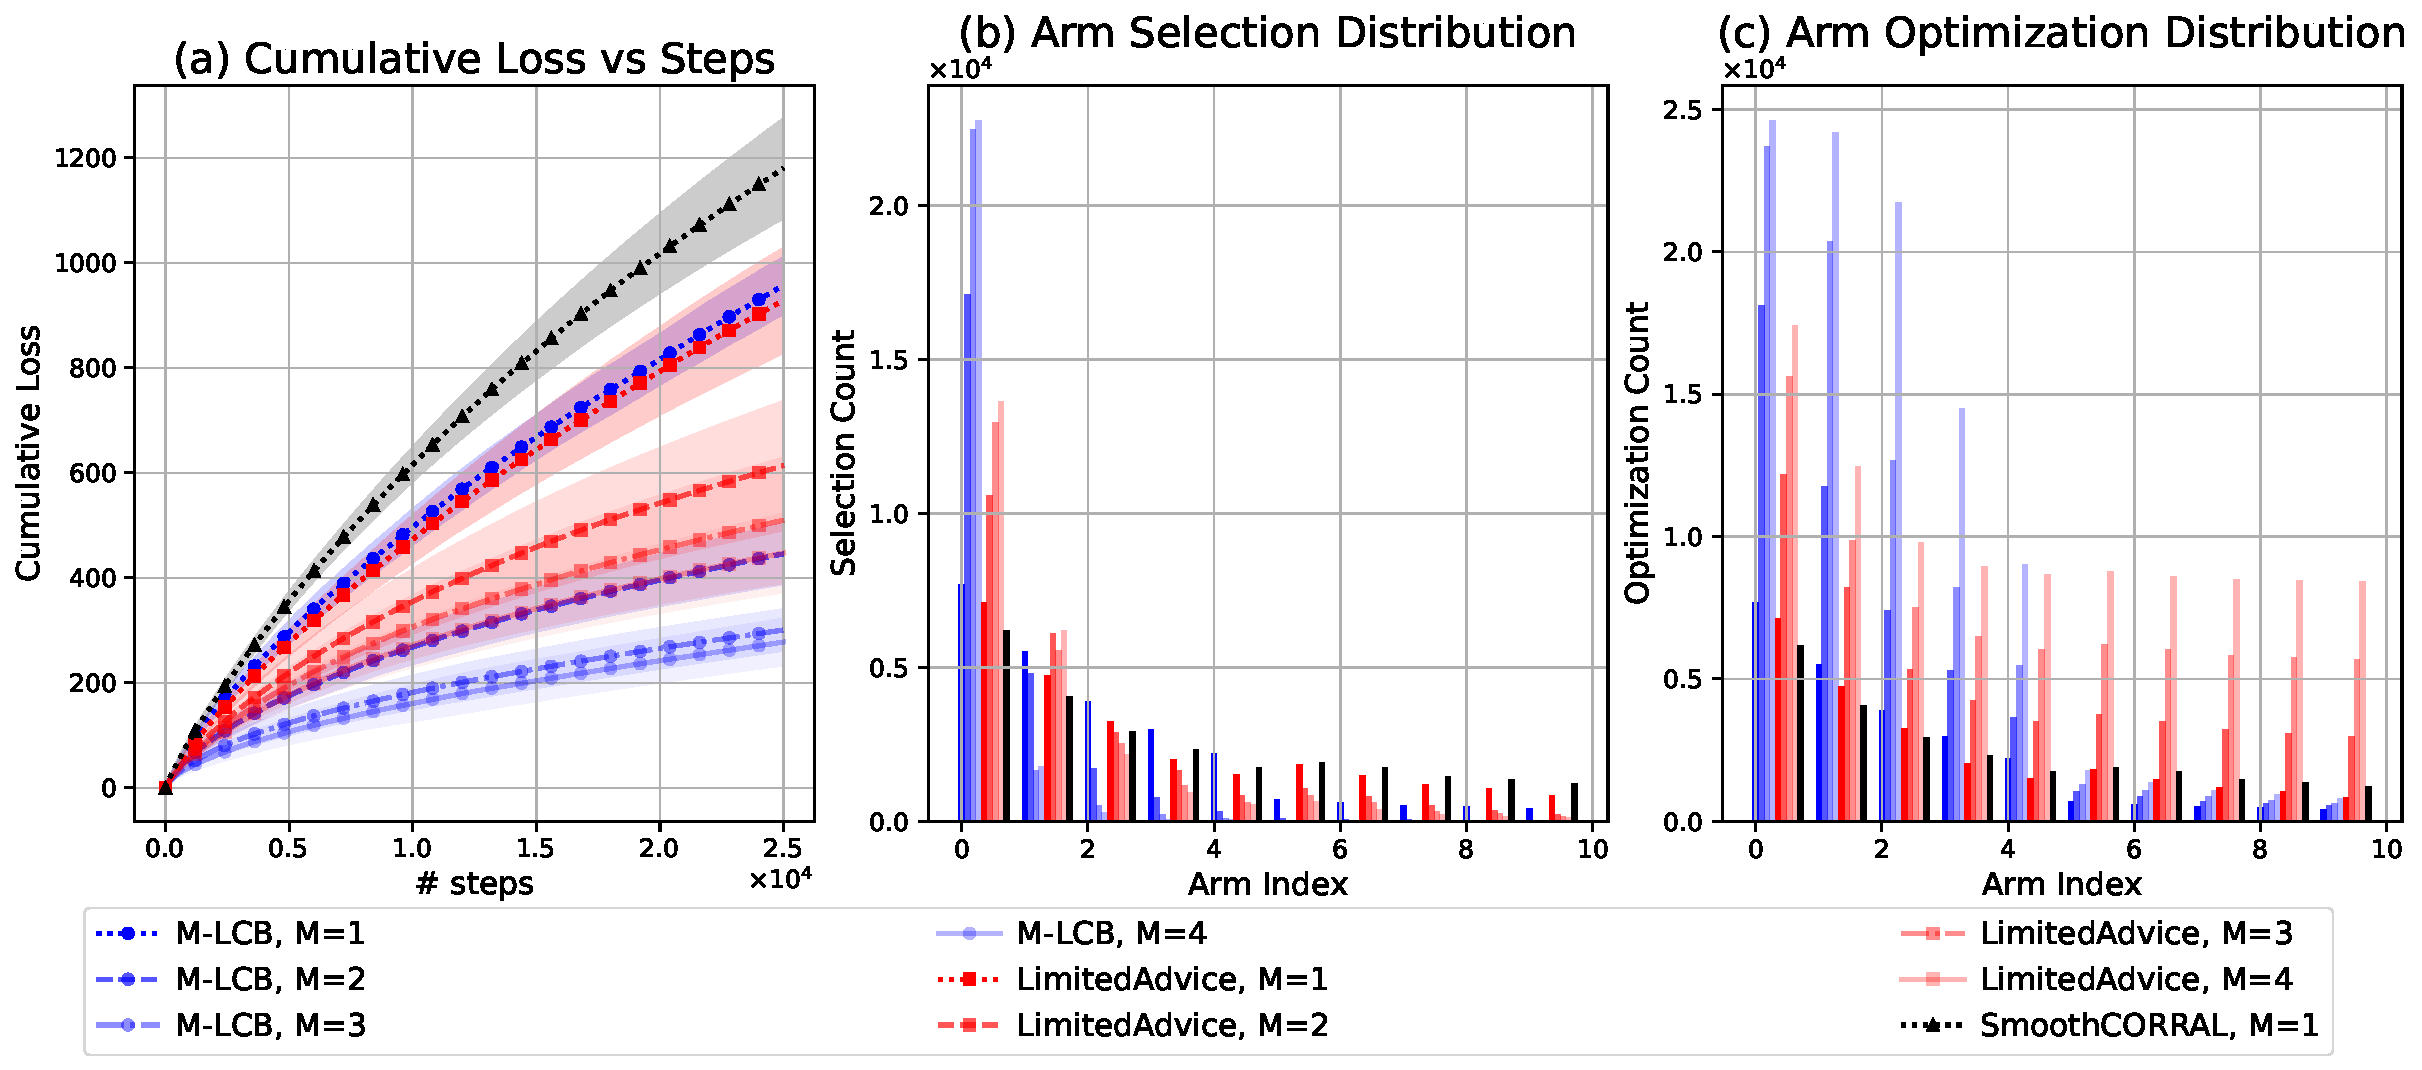
\includegraphics[width=0.75\linewidth]{figures/bandit_experiment_horizontal.pdf}
    \caption{Сравнение качества на выборе модели MAB.
    (a) Кумулятивная потеря.
    (b) Финальное распределение выбора рук.
    (c) Распределение вычислительного бюджета между руками.}
    \label{fig:regret_bandits}
\end{figure}


\vspace{-0.5em}
\section{Ограничения и будущая работа}
\vspace{-0.5em}
Наш анализ предполагает известную функцию доверительного масштабирования $c(\delta)$. В Теореме~\ref{thm:gen-rate} эта зависимость асимптотически доминируется при $\alpha < 1/2$, но становится линейной для больших $\alpha$. Будущая работа могла бы адаптировать \algname{M-LCB} к неизвестным или неверно заданным функциям масштабирования \cite{pacchiano2020model, dann2024data} и расширить схему \cite{seldin2014prediction, kveton2015tight}, чтобы включить multi-play регрет. Кроме того, вывод gap-dependent гарантий для изменяющихся во времени разрывов и исследование контекстных расширений \cite{foster2019model} представляют собой значимые технические вехи. Более подробное обсуждение ограничений приведено в Приложении \ref{sup:limitations}.

%%%%%%%%%%%%%%%%%%%%%%%%%%%%%%%%%%%%%%%%%%%%%%%%%%%%%%%%%%%%%%%%%%%%%%%%

%%% Следующие две строки задают, во-первых, стиль библиографии,
%%% и, во-вторых, используемый файл библиографии.

% \bibliographystyle{ACM-Reference-Format}
\bibliographystyle{unsrtnat}
\bibliography{lib}

%%%%%%%%%%%%%%%%%%%%%%%%%%%%%%%%%%%%%%%%%%%%%%%%%%%%%%%%%%%%%%%%%%%%%%%%


\clearpage

\appendix
\tableofcontents




\section{Обсуждение ограничений}
\label{sup:limitations}
Наш анализ предполагает, что функция доверительного масштабирования $c(\delta)$ известна. В оценке Теоремы~\ref{thm:gen-rate} эта функция появляется только через член обучения экспертов $(K/M)^{1-\alpha}T^\alpha c(\delta)$. Следовательно, при $\alpha<1/2$ этот вклад асимптотически доминируется членом исследования, тогда как для больших $\alpha$ зависимость от $c(\delta)$ линейна. Во многих стандартных экспертах, включая OGD, UCB и Hedge, $c(\delta)$ является полилогарифмической.

Случай неизвестной $c(\delta)$ рассматривается Pacchiano et al.~\cite{pacchiano2020model}, где полученные оценки регрета демонстрируют более слабую зависимость от $c(\delta)$, тогда как Dann et al.~\cite{dann2024data} оценивают ее online, получая адаптивные, но менее интерпретируемые гарантии. Поэтому адаптация \algname{M-LCB} к неизвестным или неверно заданным функциям скоростей экспертов является важным направлением будущей работы.

Другое важное направление касается алгоритмов с дополнительными наблюдениями за раунд, таких как limited-advice и multi-play bandits~\cite{seldin2014prediction,yun2018multi,kveton2015tight}.
Расширение их анализа на постановку \emph{обучаемых экспертов} объединило бы эти схемы.
% и прояснило бы роль динамики обучения при частичной обратной связи.

Еще один открытый вопрос состоит в том, можно ли получить содержательные gap-dependent логарифмические гарантии. В классических стохастических бандитах разрыв субоптимальности фиксирован, что позволяет получать оценки типа $O(\log T/\Delta)$. В нашей постановке мгновенный регрет $L(u_k^t)-L^\star$ меняется по мере обучения экспертов, поэтому релевантный разрыв зависит от времени, и прямой аналог не является немедленным.

Наконец, перспективным расширением является \emph{контекстный} режим,
где эксперты специализируются на основе наблюдаемых признаков или доменов,
что связывает нашу схему с контекстными бандитами~\cite{foster2019model}.


\section{Численные эксперименты}

Эксперименты в статье не требуют GPU. Они проводились на Macbook M1 pro с 16 gb RAM.

\subsection{Выбор модели среди обобщенных линейных моделей}
Мы оцениваем качество предложенного алгоритма \algname{M-LCB} на синтетических задачах, разработанных для проверки его способности управлять адаптивными руками при вычислительном бюджете.
Мы сравниваем с двумя базовыми методами:
\EDRB \cite{dann2024data}, алгоритмом с гарантиями для обучаемых рук,
и \algname{LimitedAdvice} \cite{seldin2014prediction}, экспертным алгоритмом, способным обрабатывать несколько обновлений рук за раунд.
Во всех экспериментах мы рассматриваем ограничения обновлений $M \in \{1,2,3\}$, усредняем результаты по 30 независимым запускам и показываем $\pm 0.5$ стандартных отклонений как заштрихованные области.

Мы рассматриваем задачу выбора модели с $K=10$ руками.
Каждая рука $k$ представляет обобщенную линейную модель (GLM) с отдельной фиксированной link function $f_k:\mathbb R\to\mathbb R$.
На каждом раунде $t$ вектор признаков $x_t \in \mathbb R^d$ выбирается равномерно с единичной сферы $\mathbb S^{d-1}$,
а метка генерируется оптимальной рукой $k^\star=9$ как
\begin{equation}
r_t = f_{k^\star}(w^\top x_t),
\end{equation}
Как показано на Рисунке~\ref{fig::glm_functions}, link functions $f_7, f_8,$ и $f_9$ весьма похожи в областях, где данные плотны,
что создает нетривиальную задачу исследования.

\begin{figure}
    \centering
    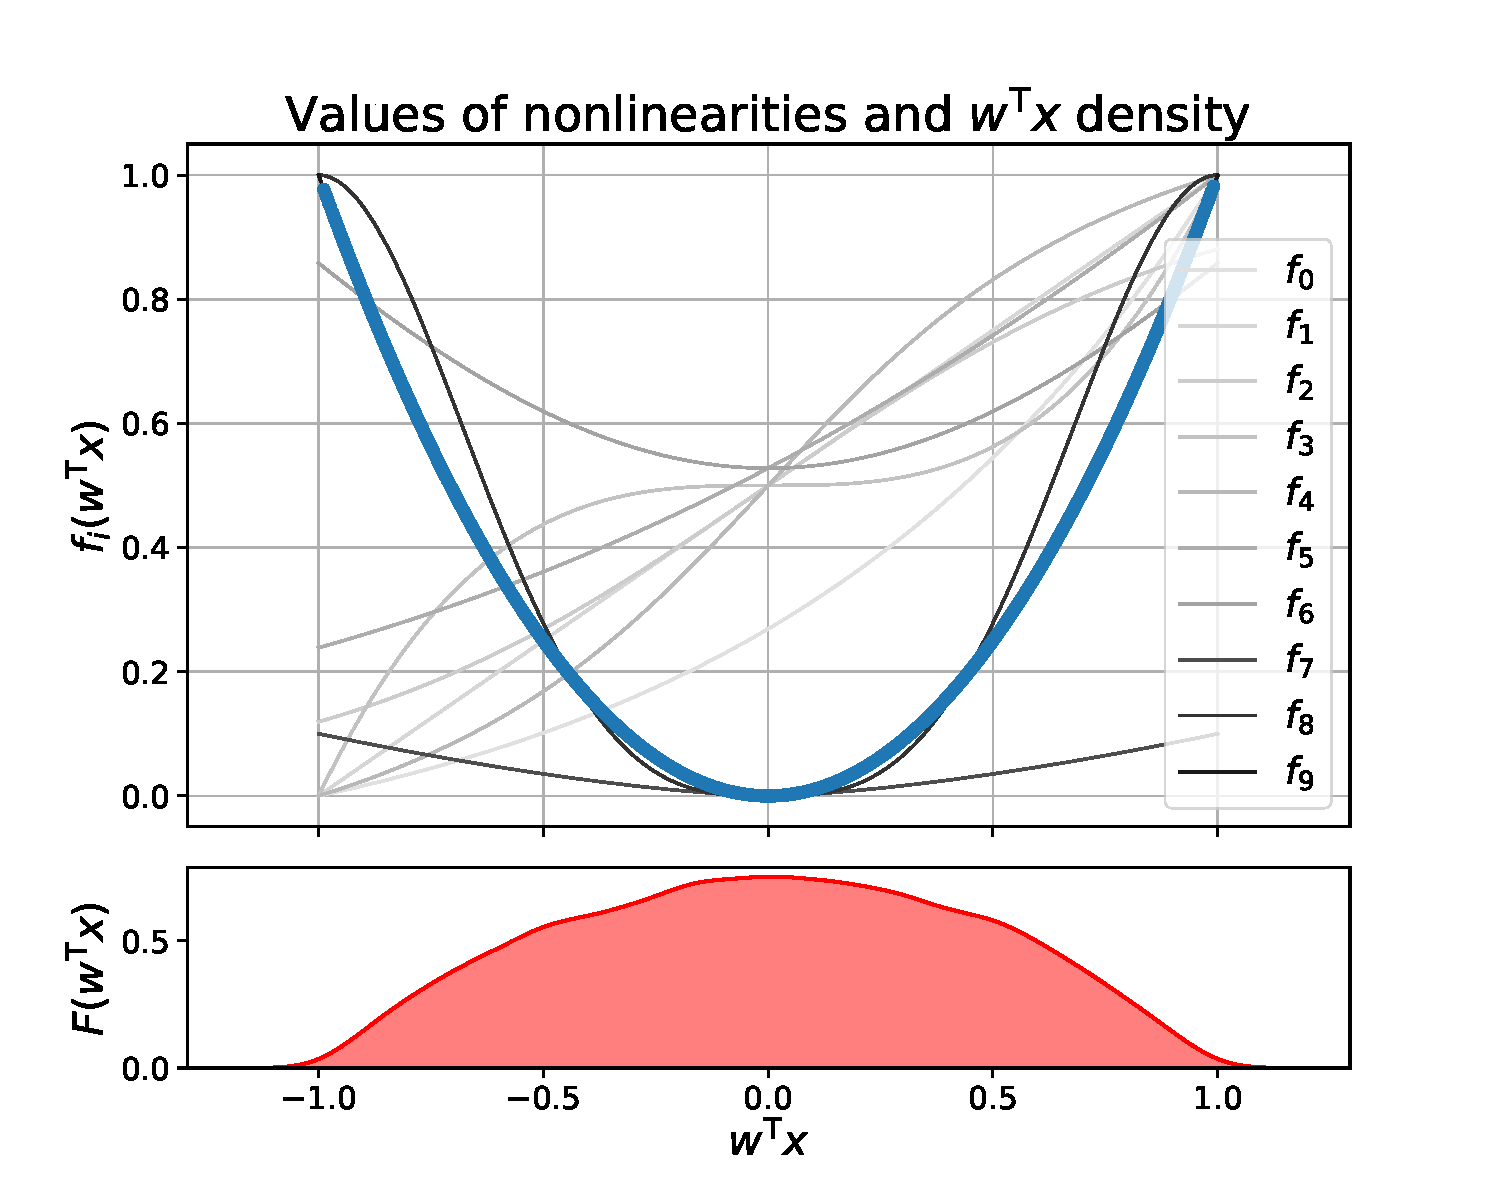
\includegraphics[width=0.5\linewidth]{figures/nonlinearities_image.pdf}
    \caption{Нелинейные link functions, связанные с руками (сверху), и плотность сгенерированных точек данных (снизу).
    Видно, что последние три функции весьма похожи там, где данные сконцентрированы, что затрудняет различение оптимальной руки.}
    \label{fig::glm_functions}
\end{figure}

\paragraph{Результаты.}
Рисунок~\ref{fig:exp2} суммирует результаты.
Панель (a) показывает, что \algname{M-LCB} достигает сублинейного регрета и конкурентоспособен с обоими базовыми методами.
Панель (b) сообщает финальное распределение выбора рук: \algname{M-LCB} успешно идентифицирует оптимальную руку ($k=9$).
Панель (c) представляет распределение вычислительного бюджета между руками.
\algname{M-LCB} распределяет обновления преимущественно на лучшие по качеству руки, тогда как \algname{LimitedAdvice} распределяет обновления более равномерно, что приводит к менее эффективному использованию бюджета обучения.

\begin{figure}[!ht]
    \centering
    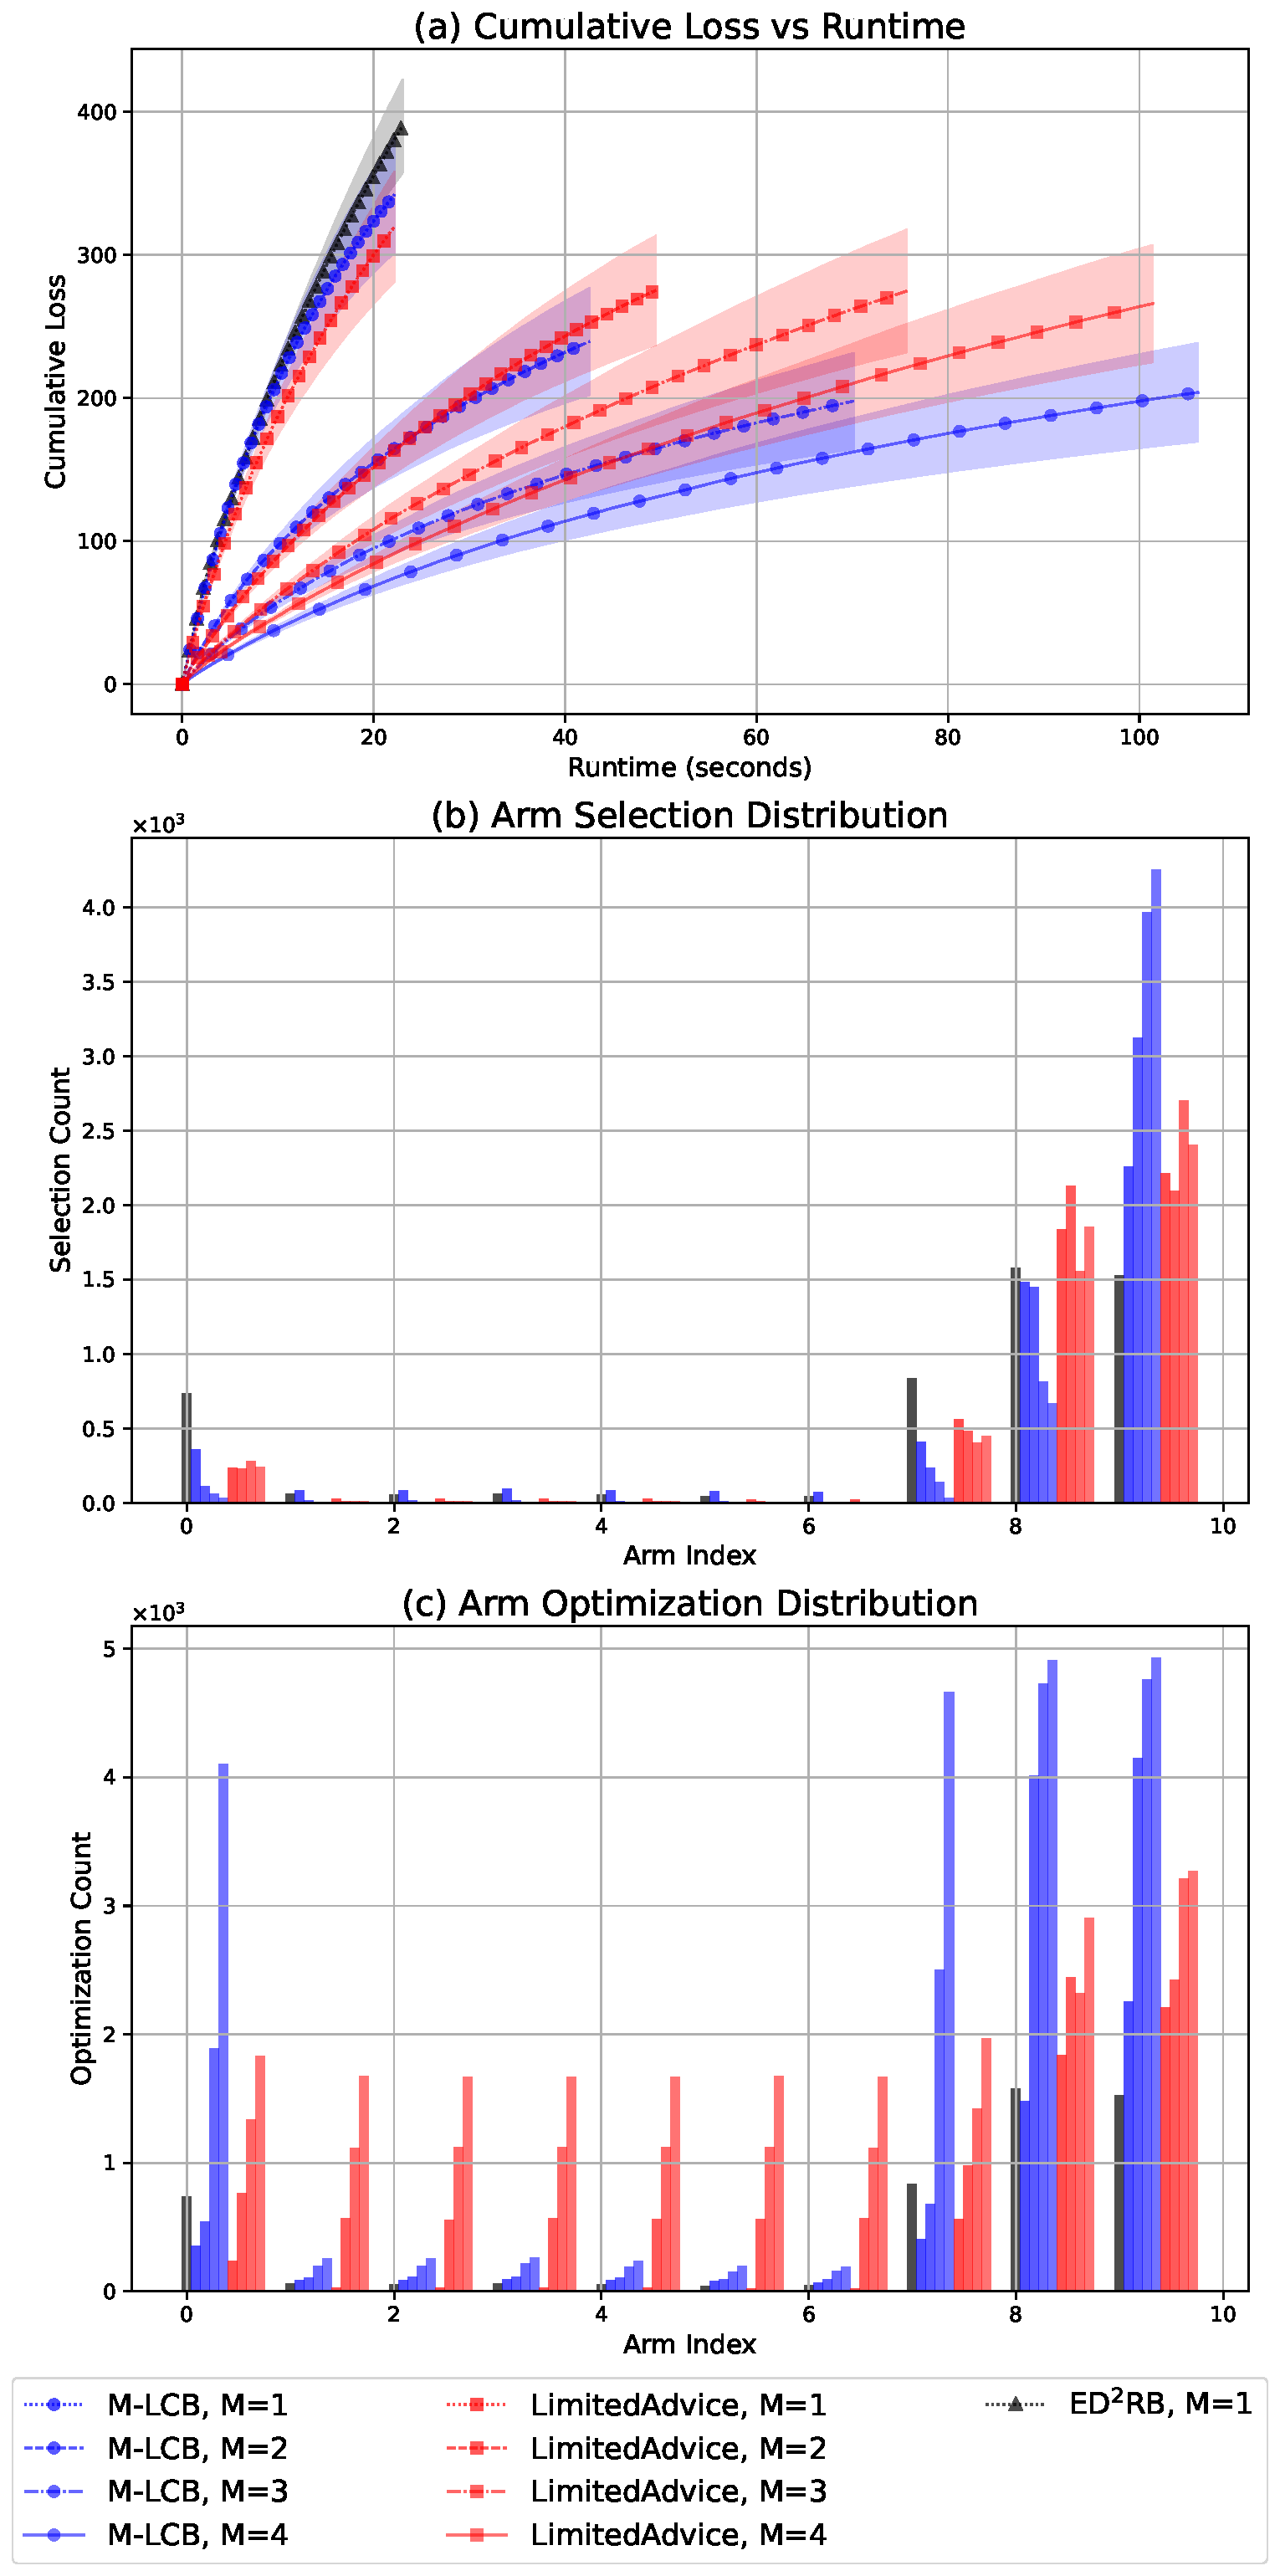
\includegraphics[width=0.8\linewidth]{figures/regrets_image.pdf}
    \caption{Сравнение качества на задаче выбора GLM-модели.
    (a) Кумулятивный регрет.
    (b) Финальное распределение выбора рук.
    (c) Распределение вычислительного бюджета между руками.}
    \label{fig:exp2}
\end{figure}

\subsubsection*{Гиперпараметры}
Для \EDRB параметр исследования подбирался, причем $c=0.1$ давал лучшие результаты.
Для \algname{M-LCB} концентрационные члены были один раз настроены в валидационной среде.
Параметры для \algname{LimitedAdvice} задавались согласно его теоретическому анализу \cite{seldin2014prediction}. Анализ показывает, что регрет не очень чувствителен к этим параметрам.


\subsection{Online-выбор бандитных алгоритмов}

В этом эксперименте мы конкретизируем нашу схему для решения задачи выбора модели, где каждый эксперт $k \in [K]$ сам является независимым стохастическим алгоритмом Multi-Armed Bandit (MAB).

\begin{figure}[!ht]
    \centering
    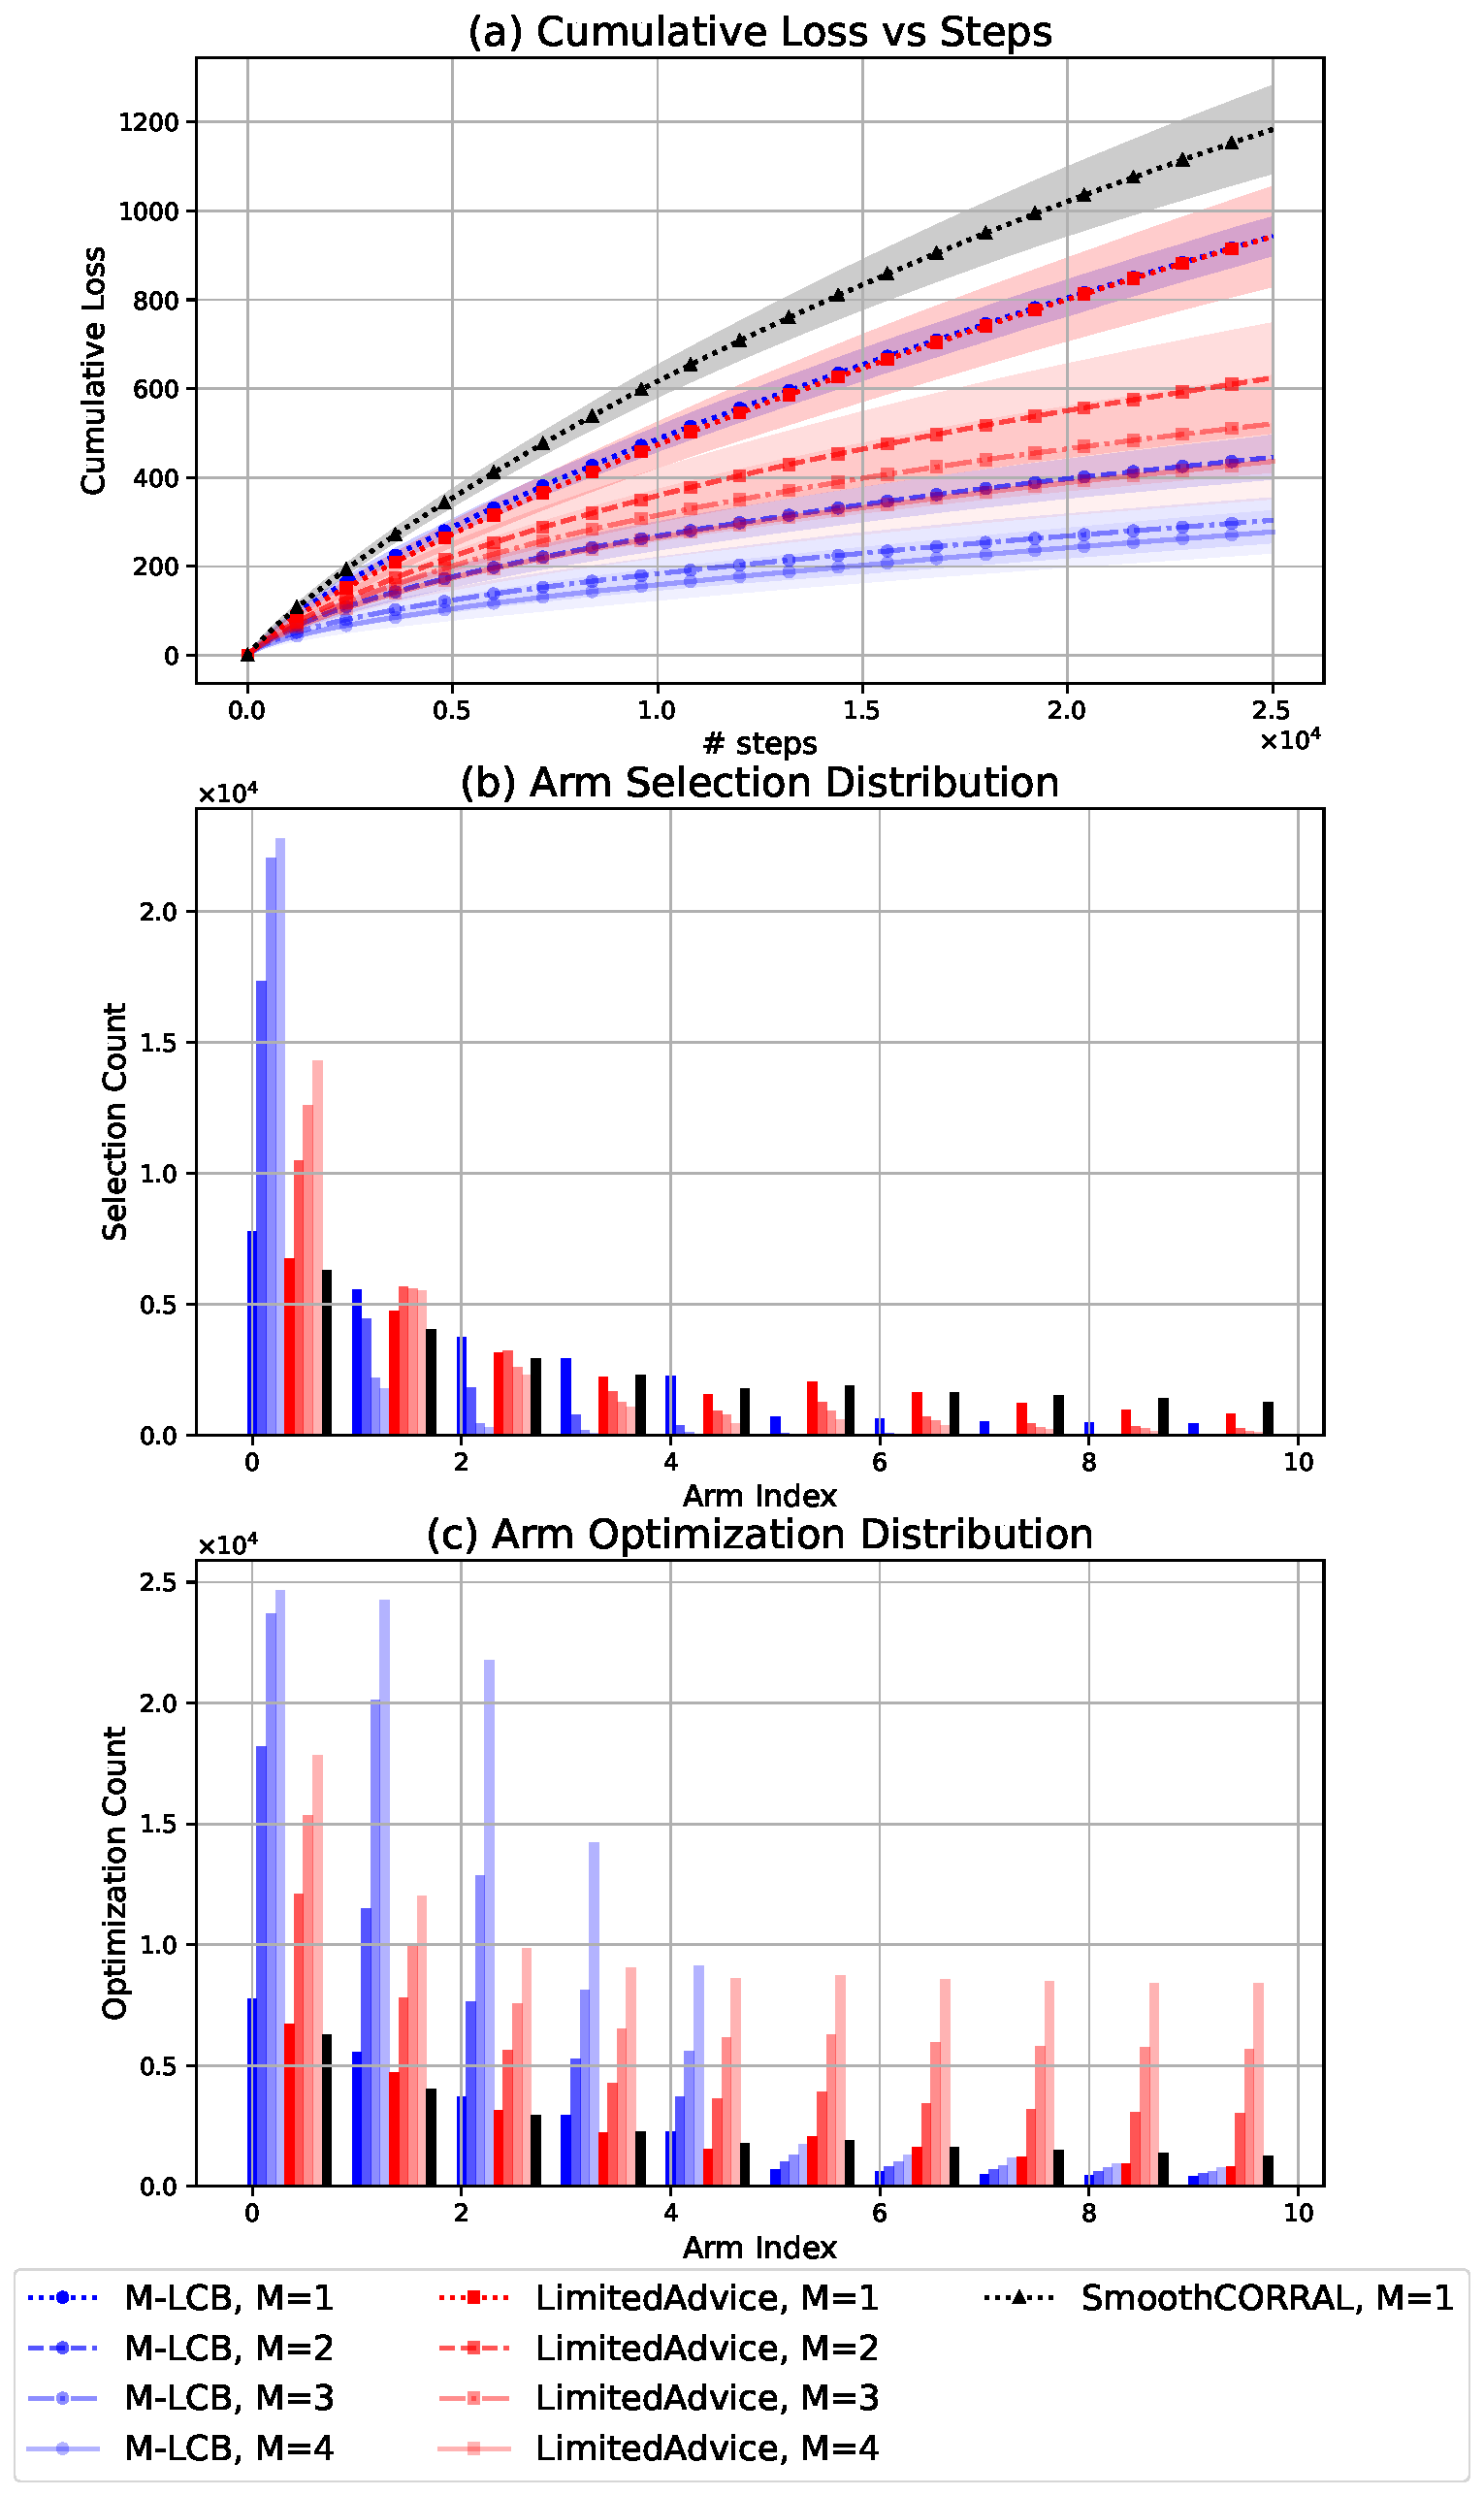
\includegraphics[width=0.8\linewidth]{figures/bandit_experiment.pdf}
    \caption{Сравнение качества на выборе модели MAB.
    (a) Кумулятивный регрет.
    (b) Финальное распределение выбора рук.
    (c) Распределение вычислительного бюджета между руками.}
    \label{fig:regret_bandits_appendix}
\end{figure}


\begin{table*}[h!]
\centering
\caption{%
Примеры скоростей сходимости внутренних рук $U_k(n,\delta)$ и соответствующего глобального регрета (с точностью до логарифмических множителей и аддитивного члена $O(\sqrt{(K/M)T})$).
Для каждого эксперта $k$ внутренний алгоритм удовлетворяет $U_k(t,\delta)=O(\beta_k\,t^{\alpha}c(\delta))$,
а соответствующий глобальный регрет масштабируется как
$O\!\big(T^{\alpha}c(\delta)\,\|{\boldsymbol{\beta}}\|_{M, 1-\alpha}\big)$,
где
$\|{\boldsymbol{\beta}}\|_{M,\gamma}
=\Bigl(\tfrac{1}{M}\sum_{k=1}^{K}\beta_k^{\frac{1}{\gamma}}\Bigr)^{\gamma}$.
Соглашения о параметрах:
$K$ — \# экспертов; $M$ — бюджет обучения на раунд; $T$ — горизонт;
$N_k$ — \# базовых рук/действий; $d_k$ — размерность признаков;
$\varepsilon$ — показатель момента для тяжелых хвостов ($\mathbb{E}|X|^{1+\varepsilon}\!\le\sigma^{1+\varepsilon}$);
$L, R, C, G$ — липшицева константа, диаметр, диапазон и градиентные константы.
}
\label{tab:convergence_examples}
\begin{tabular}{p{5.0cm}p{3.7cm}p{4.0cm}}
\toprule
\textbf{Внутренний алгоритм / задача}
& \textbf{Внутренняя скорость $U_k(n,\delta)$}
& \textbf{Глобальный регрет (с точностью до log)} \\
\midrule
OGD / OMD (convex Lipschitz)
& $O(G_kR_k\sqrt{n})$, $\alpha=\tfrac{1}{2}$,
& $O\!\big(T^{1/2}\,\|GD\|_{M,1/2}\big)$ \\

\midrule
Bandit Convex Optimization (bounded $f_t$)~\cite{flaxman2004online}
& $O(C_kd_kn^{5/6})$, $\alpha=\tfrac{5}{6}$
& $O\!\big(T^{5/6}\,\|Cd\|_{M,1/6}\big)$ \\

\midrule
Bandit Convex Optimization ($L$–Lipschitz $f_t$)~\cite{flaxman2004online}
& $O(\sqrt{C_kL_kR_k}d_kn^{3/4})$, $\alpha=\tfrac{3}{4}$
& $O\!\big(T^{3/4}\,\|\sqrt{CLR}d\|_{M,1/4}\big)$ \\

\midrule
Heavy–tailed stochastic bandits~\cite{bubeck2013bandits}
& $\tilde O(n^{\alpha}N_k^{1-\alpha})$, $\alpha=\tfrac{1}{1+\varepsilon}$
& $O\!\big(T^{\alpha}\, [\frac{1}{M}\sum_{k=1}N_k]^{1 - \alpha})$ \\
% $\|N^{1-\alpha}\|_{M,1 -\alpha}\big)$ \\

\midrule
Heavy–tailed stochastic bandits (Symmetric noise)~\cite{dorn2024fast}
& $O(\sqrt{N_k n} {\log n}^{\frac{3}{2}})$, $\alpha=\tfrac{1}{2}$
& $O\!\big(T^{1/2}\,[\frac{1}{M}\sum_{k=1}N_k]^\frac{1}{2}\big)$ \\

\midrule
Heavy–tailed linear bandits~\cite{tajdini2025improved}
& $O(d_k^{\frac{3}{2} - \alpha} n^{\alpha})$, $\alpha=\tfrac{1}{1 + \varepsilon}$
& $O\big(T^{\alpha}\,\|d^{\frac{3}{2} - \alpha}\|_{M,1 - \alpha}\big)$ \\

\midrule
Hedge / Exponential Weights (over $N_k$ experts)
& $O(\sqrt{n\log N_k})$, $\alpha=\tfrac{1}{2}$,
& $O\!\big(T^{1/2}\,\|\sqrt{\log N}\|_{M,1/2}\big)$ \\
\bottomrule
\end{tabular}
\end{table*}

\subsection{Эксперименты на реальных данных}
\label{sup:real_data}

Мы дополнительно оцениваем \algname{M-LCB} на двух реальных многоклассовых клинических бенчмарках предсказания, которые нагружают разные аспекты постановки с ограниченной обратной связью. Первый бенчмарк проверяет поведение регрета на длинном горизонте через bootstrapped поток из фармакогеномного датасета среднего размера, тогда как второй использует полностью реальный, non-bootstrapped поток для оценки качества при повторных случайных порядках меньшего медицинского мониторингового датасета.
\paragraph{Дозирование варфарина.}
Сначала мы рассматриваем датасет дозирования варфарина IWPC \cite{international2009estimation, bastani2020mostly}, содержащий 5,528 пациентов, 93 признака и трехклассовую метку дозировки. Поскольку датасет меньше горизонта, необходимого для выявления асимптотических трендов регрета, мы генерируем поток из $T=20{,}000$ раундов с помощью bootstrap resampling. Пул экспертов состоит из $K=7$ неоднородных online softmax и perceptron классификаторов, построенных с использованием разных классов моделей и подмножеств признаков. Мы сравниваем методы при бюджетах обновлений $M\in\{1,2,4\}$.

Результаты подтверждают предсказанную зависимость от бюджета советов. Как показано на Рисунке~\ref{fig:warfarin_theoretical}, \algname{M-LCB} получает наименьшую кумулятивную потерю среди сравниваемых online-методов. Например, при $M=2$ \algname{M-LCB} достигает кумулятивной потери $6{,}604$, близкой к best-fixed-expert reference $6{,}589$. Этот малый разрыв указывает, что, несмотря на наблюдение и обновление только ограниченного числа экспертов за раунд, алгоритм быстро концентрирует обновления на конкурентоспособных экспертах и отслеживает лучший фиксированный компаратор. Мы также варьируем число экспертов $K\in\{7,10,15\}$ при фиксированном $M=2$. Рисунок~\ref{fig:warfarin_scaling} показывает, что регрет растет с $K$, что согласуется с зависимостью $\mathcal{O}(\sqrt{KT/M})$ в Теореме~\ref{thm:gen-rate-topM}.

\begin{figure}[t]
    \centering
    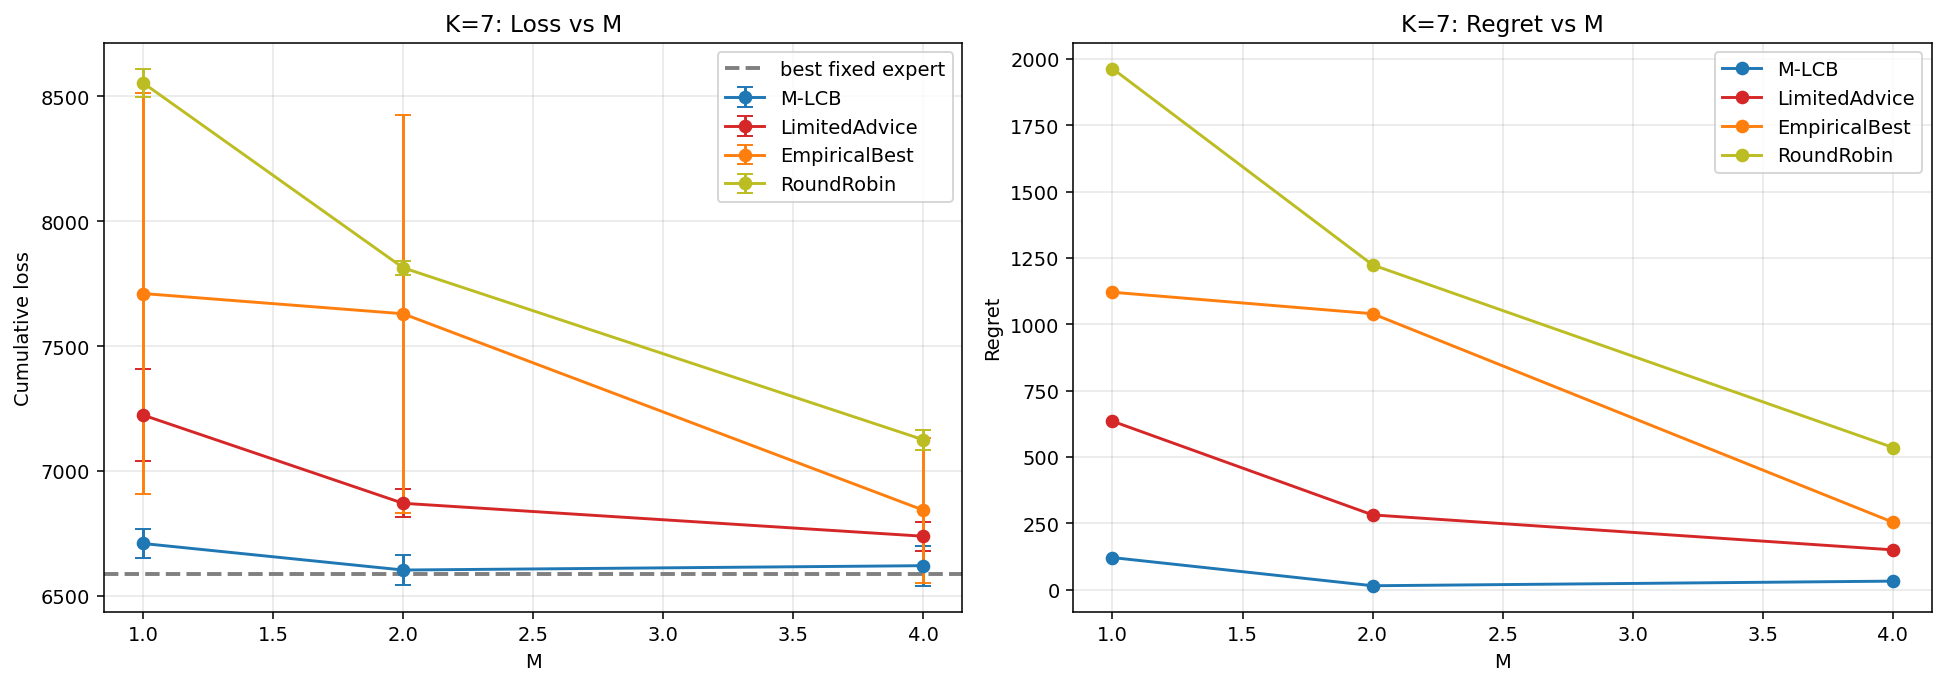
\includegraphics[width=0.95\linewidth]{figures/Warfarian_Dosage_theoretical.png}
    \caption{Результаты дозирования варфарина при ограниченных бюджетах советов. \algname{M-LCB} достигает наименьшей кумулятивной потери среди сравниваемых методов и при $M=2$ получает кумулятивную потерю $6{,}604$, близкую к best-fixed-expert reference $6{,}589$.}
    \label{fig:warfarin_theoretical}
\end{figure}

\begin{figure}[t]
    \centering
    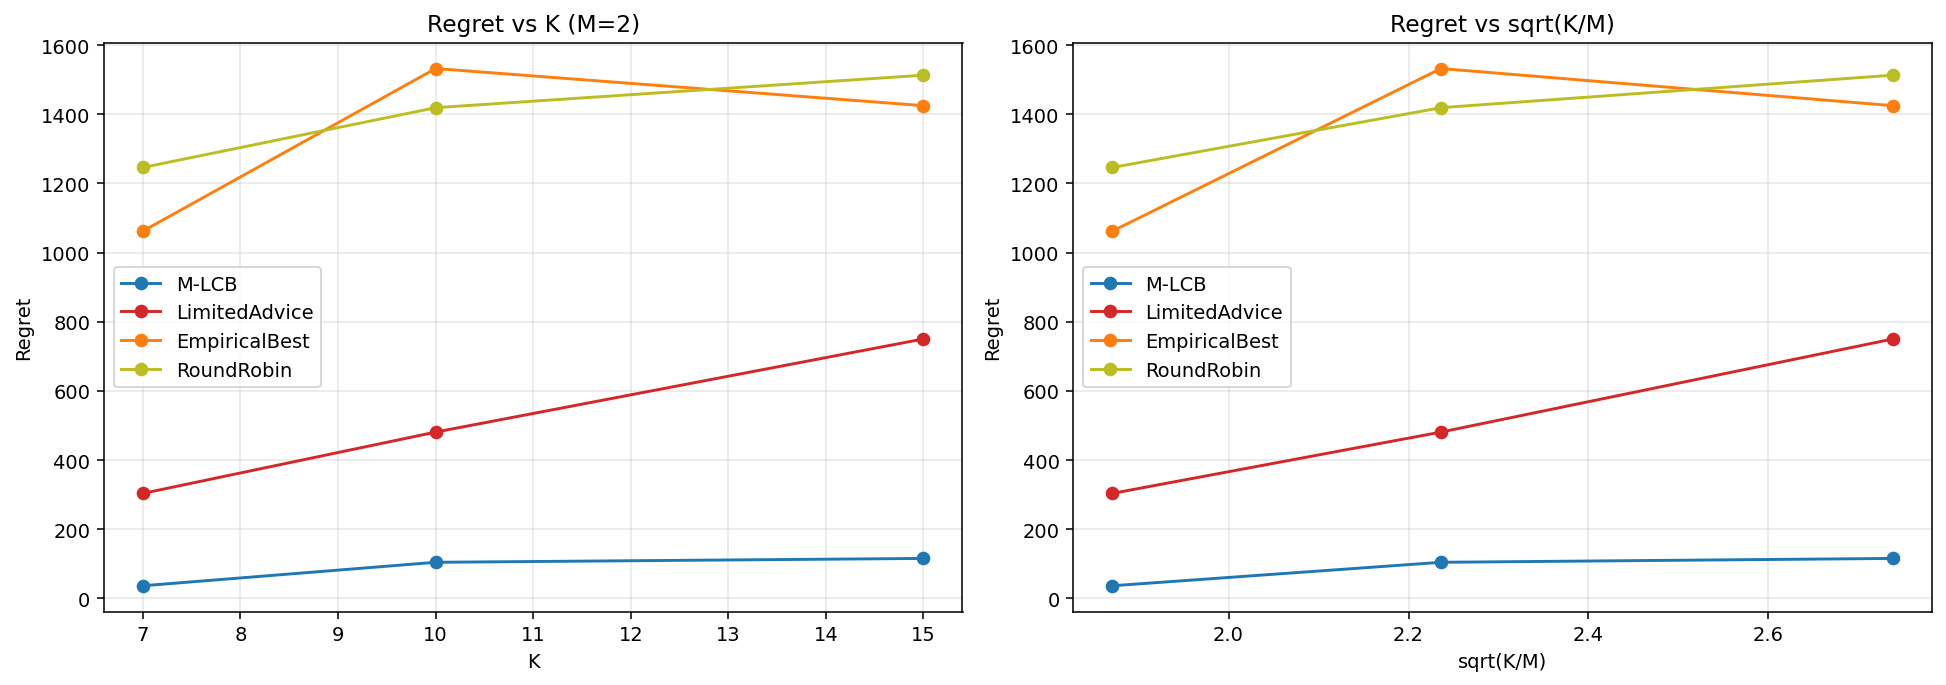
\includegraphics[width=0.95\linewidth]{figures/Warfarian_Dosage_scaling.png}
    \caption{Поведение масштабирования на бенчмарке дозирования варфарина при $K\in\{7,10,15\}$ и фиксированном бюджете $M=2$. Регрет растет с числом экспертов, что соответствует качественному предсказанию зависимости регрета $\mathcal{O}(\sqrt{KT/M})$.}
    \label{fig:warfarin_scaling}
\end{figure}

\begin{figure}[h!t]
    \centering
    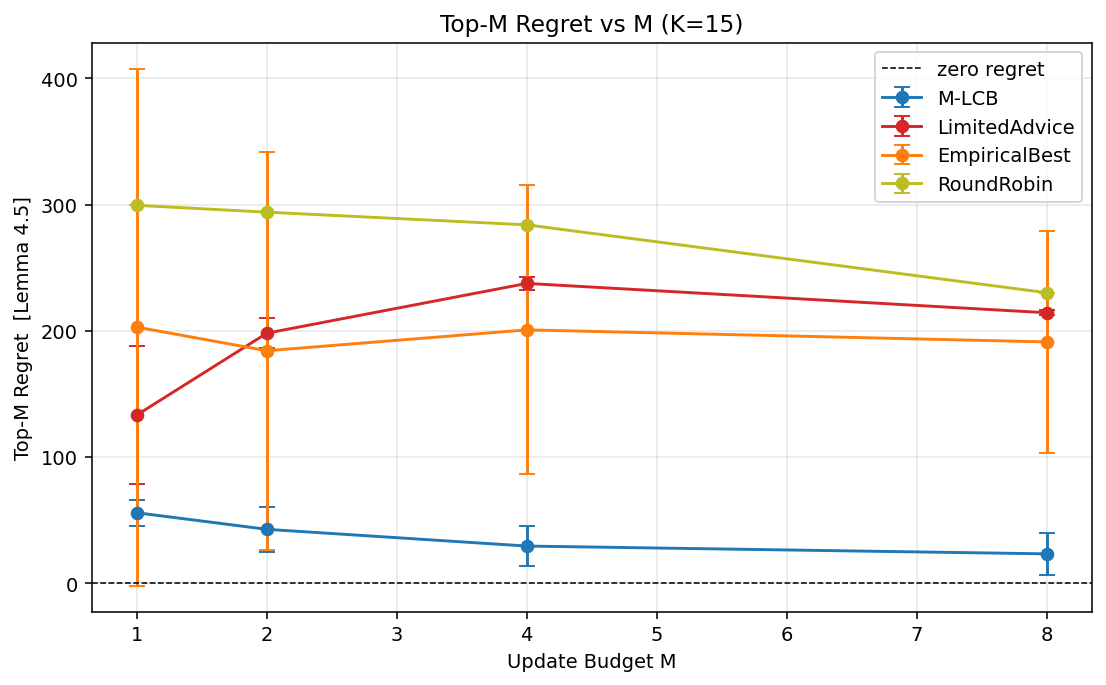
\includegraphics[width=0.8\linewidth]{figures/Cardiotocography_topM.png}
    \caption{Top-$M$ регрет на бенчмарке Cardiotocography при $K=15$ экспертах и бюджетах $M\in\{1,2,4,8\}$ по 20 random seeds. При $M\ge4$ \algname{M-LCB} получает почти нулевой top-$M$ регрет, совпадая с лучшим фиксированным подмножеством из $M$ экспертов.}
    \label{fig:ctg_topm}
\end{figure}

\paragraph{Cardiotocography.}
Далее мы оцениваем на датасете Cardiotocography \cite{cardiotocography_193, bastani2020mostly}, содержащем 2,126 записей фетального мониторинга, 35 признаков и трехклассовую метку состояния плода. В отличие от эксперимента с Warfarin, этот бенчмарк использует полностью реальный, non-bootstrapped поток. Мы используем пул экспертов с $K=15$ экспертами и варьируем бюджет советов по $M\in\{1,2,4,8\}$ на 20 random seeds.


Экспериментальные результаты на датасете Cardiotocography показывают, что качество обученной смеси монотонно улучшается с ростом бюджета обновлений.
При конфигурации $M=4$ \algname{M-LCB} достигает $95.0\%$ средней accuracy и $105.6$ кумулятивной потери; для сравнения, оптимальный фиксированный эксперт достигает потери $86.0$.
Рисунок~\ref{fig:ctg_topm} показывает top-$M$ регрет, где \algname{M-LCB} стабильно превосходит \algname{LimitedAdvice}, \algname{RoundRobin} и \algname{SmoothCORRAL}.
Это различие в качестве подчеркивает эффективность адаптивного распределения бюджета по сравнению со статическими или стохастическими политиками обновления.
Примечательно, что наблюдение о работе \algname{M-LCB} на уровне лучшего фиксированного подмножества из $M$ экспертов дает сильное эмпирическое подтверждение теоретической гарантии на уровне подмножеств, представленной в Теореме~\ref{thm:gen-rate-topM}.


\section{Примеры использования}

\subsection{Алгоритмы многоруких бандитов как эксперты.}
\label{sup:bandit_application}
 Мотивированные AutoML и распределенной маршрутизацией, мы рассматриваем мета-процедуру $\mathcal{P}$, выбирающую наиболее эффективного среди $K$ самооптимизирующихся экспертов. Как и в Bandit Model Selection \cite{pacchiano2020model}, это по своей природе сложно из-за нестационарной динамики обучения экспертов и высокой стоимости выборок, требуемой для сходимости.

Каждый эксперт $k$ является стохастическим бандитом, управляющим конечным пространством действий $\mathcal{A}_k := \{a_k^1, \dots, a_k^{m_k}\}$. Решение эксперта в момент $t$ — распределение вероятностей $u_k^t \in \Delta_k$ по его действиям, где $\mathbf{U}_k = \Delta_k$ — $m_k$-мерный симплекс. Глобальное пространство решений $\mathbf{U}$ является объединением симплексов.


Среда характеризуется латентной случайной величиной $\xi^t \sim D$, представляющей состояние системы в момент $t$ (например, вектор текущих задержек или ресурсных затрат для всех доступных методов). Хотя $\xi^t$ не обязательно полностью наблюдается мета-процедурой, она определяет потерю каждого действия $a \in \bigcup_k \mathcal{A}_k$ через отображение $\tilde{\ell}(a, \xi)$.
Потеря эксперта для решения $u_k \in \mathbf{U}_k$ равна $\ell(u_k, \xi) := \mathbb{E}_{a \sim u_k} [\tilde{\ell}(a, \xi)]$. Оптимальный риск эксперта $k$ равен $L_k^\star = \min_{a \in \mathcal{A}_k} \mathbb{E}_{\xi \sim D} [\tilde{\ell}(a, \xi)]$.

Когда эксперт $k\in S_t$ выдает $u^{t}_k$, он семплирует дискретное действие $a_k^{t} \in \mathcal{A}_k$ из $u_k^{t}$ и получает $(a^{t}_k, \tilde{\ell}(a^{t}_k, \xi^{t}))$ как бандитную обратную связь. Таким образом, в этой конкретизации предположение limited-advice означает, что среда предоставляет потерю семплированного действия для каждого обучаемого эксперта $k\in S_t$, включая экспертов, которые не развернуты как глобальный советчик. Если несколько обучаемых экспертов семплируют одно и то же действие, соответствующую потерю достаточно вычислить один раз и можно переиспользовать для всех них. Когда доступны off-policy обновления, можно также обновлять базовые алгоритмы по дополнительным выборкам, но наш анализ использует только указанные выше on-policy наблюдения.

В этой постановке качество эксперта измеряется его псевдо-регретом $R_k(n)$, который оценивает кумулятивную ожидаемую потерю распределений $u_k^\tau$ относительно лучшего фиксированного действия, $R_k(t) = \sum_{\tau \in I_k(t)} \mathbb{E}_{a \sim u_k^\tau} [\tilde{\ell}(a, \xi^\tau)] - n_k L_k^\star.$

Стандартные алгоритмы, такие как \algname{UCB}, удовлетворяют Asm.~\ref{assumption:expert_regret} с $U_k(n, \delta) = O(\sqrt{m_k n \log(n/\delta)})$. Теоретическая накопленная потеря $L_k(t)$ в~\eqref{def:experts_running_loss} определяется через условную потерю $\ell(u_k^t,\xi^t)$, тогда как бандитный эксперт наблюдает семплированную потерю $\tilde{\ell}(a_k^t,\xi^t)$. Поэтому в реализации используется $\tilde L_k(t)=\frac{1}{n_k^t}\sum_{\tau\in I_k(t)}\tilde{\ell}(a_k^\tau,\xi^\tau),$
и к $U_k$ добавляется соответствующий концентрационный член для семплирования. Концентрация $\sum_{\tau\in I_k(t)} \tilde{\ell}(a_k^\tau, \xi^\tau)$ вокруг $\sum_{\tau\in I_k(t)} \ell(u_k^\tau, \xi^\tau)$ обеспечивает anytime высоковероятностные границы на псевдо-регрет. Доказательство аналогично Лемме~\ref{lem:prefix_to_expected}.


\subsection{Конкретные примеры}
\label{sup:applications}
Таблица~\ref{tab:convergence_examples} суммирует несколько репрезентативных базовых алгоритмов, их внутренние скорости сходимости и результирующий глобальный регрет при объединении с \algname{M-LCB}.
Наряду со стандартными выпуклыми и exponentially-weighted обучающимися алгоритмами мы включаем ``трудные'' стохастические задачи с тяжелохвостыми наградами, которые демонстрируют более медленную сходимость, характеризуемую большим $\alpha$.

Разные эксперты могут действовать на различных пространствах действий.
Например, в bandit-based экспертах каждый обучающийся алгоритм может контролировать собственный набор рук, тогда как в параметрических или линейных моделях размерность пространства признаков может различаться. Такая неоднородность отражается в параметрах типа $N_k$ или $d_k$ в Таблице~\ref{tab:convergence_examples} и естественно обрабатывается в рамках \algname{M-LCB}.



\section{Доказательства}


\begin{lemma}[Связь OCO-регрета с регретом эксперта]
\label{lem:prefix_to_expected}
Рассмотрим эксперта $k$, описанного в Разделе~\ref{sec:examples_parametric}. Предположим, что эксперт предоставляет anytime высоковероятностную оценку $\overline{U}_k(t, \delta)$ для OCO-регрета $\overline{R}_k(t)$, определенного в \eqref{eq:regret_oco}. То есть для любого фиксированного $\delta \in (0,1)$:
$
    \mathbb{P}\left( \forall t \ge 1, \quad \overline{R}_k(t) \le \overline{U}_k(t, \delta) \right) \ge 1 - \delta.
$
Тогда эксперт удовлетворяет Asm.~\ref{assumption:expert_regret} относительно регрета $R_k(t)$ с оценкой:
\begin{equation*}
U_k(t, \delta) = \overline{U}_k(t, \delta/2) + t \cdot G(t, \delta/(3.5t^2)),
\end{equation*}
где $G(t, \delta)$ — концентрационный член:
\begin{equation*}
G(t, \delta) = \sqrt{\frac{2 \log(1/\delta)}{t}} + \frac{2 \log(1/\delta)}{3t}.
\end{equation*}
\end{lemma}

\begin{proof}
Для любого времени $t$ пусть $n = |I_k(t)|$ обозначает число раундов, на которых эксперт $k$ обновлялся. Для упрощения обозначений мы перенумеруем обучающие раунды эксперта $k$ как $\tau = 1, \dots, n$ и обозначим соответствующие решения и потери как $u_k^\tau$ и $\xi^\tau$ соответственно.
Зафиксируем $\delta \in (0, 1)$ и определим концентрационный член $G(n, \delta') = \sqrt{\frac{2 \log(1/\delta')}{n}} + \frac{2 \log(1/\delta')}{3n}$.

Мы определяем два высоковероятностных события. Сначала пусть $\mathcal{E}_1$ — событие, на котором выполняется anytime OCO-оценка регрета для эксперта $k$. По предположению Леммы с вероятностью не менее $1 - \delta/2$:
\begin{equation}
\label{eq:emp_reg_proof}
    \sum_{\tau=1}^n \ell(u_k^\tau, \xi^\tau) - \min_{u \in \mathbf{U}_k} \sum_{\tau=1}^n \ell(u, \xi^\tau) \le \overline{U}_k(n, \delta/2) \quad \forall n \ge 1.
\end{equation}

Во-вторых, пусть $u_k^\star \in \arg \min_{u \in \mathbf{U}_k} L(u)$ — оптимальное фиксированное решение по ожиданию, так что $L(u_k^\star) = L_k^\star$. Применяя Asm.~\ref{assumption:stochastic_losses} и Лемму~\ref{lem:loss-eval} к последовательности i.i.d. потерь $\{\ell(u_k^\star, \xi^\tau)\}_{\tau=1}^n$, получаем, что для фиксированного $n$ с вероятностью не менее $1 - \delta/(3.5n^2)$:
\begin{equation*}
    \frac{1}{n} \sum_{\tau=1}^n \ell(u_k^\star, \xi^\tau) \le L_k^\star + G\bigl(n, \delta / (3.5n^2)\bigr).
\end{equation*}
Беря union bound по всем $n \ge 1$ и отмечая, что $\sum_{n=1}^\infty \frac{1}{3.5n^2} = \frac{1}{3.5} \frac{\pi^2}{6} < 0.5$, определим $\mathcal{E}_2$ как событие, на котором это неравенство выполняется одновременно для всех $n$. Следовательно, $\mathbb{P}(\mathcal{E}_2) \ge 1 - \delta/2$, и на $\mathcal{E}_2$ для всех $n \ge 1$ выполнено
\begin{equation}
\label{eq:comp_conc_proof}
    \sum_{\tau=1}^n \ell(u_k^\star, \xi^\tau) \le n L_k^\star + n G\bigl(n, \delta / (3.5n^2)\bigr).
\end{equation}

По union bound, $\mathbb{P}(\mathcal{E}_1 \cap \mathcal{E}_2) \ge 1 - \delta$. На этом пересечении мы используем оптимальность эмпирического минимизатора и замечаем, что $\min_{u \in \mathbf{U}_k} \sum_{\tau=1}^n \ell(u, \xi^\tau) \le \sum_{\tau=1}^n \ell(u_k^\star, \xi^\tau)$. Объединяя \eqref{eq:emp_reg_proof} и \eqref{eq:comp_conc_proof}, получаем для всех $n \ge 1$:
\begin{align*}
    \sum_{\tau=1}^n \ell(u_k^\tau, \xi^\tau) &\le \min_{u \in \mathbf{U}_k} \sum_{\tau=1}^n \ell(u, \xi^\tau) + \overline{U}_k(n, \delta/2) \\
    &\le \sum_{\tau=1}^n \ell(u_k^\star, \xi^\tau) + \overline{U}_k(n, \delta/2) \\
    &\le n L_k^\star + \overline{U}_k(n, \delta/2) + n G\bigl(n, \delta / (3.5n^2)\bigr).
\end{align*}

Наконец, переставляя члены последнего неравенства, получаем неравенство как в Предположении \ref{assumption:expert_regret}. Это завершает доказательство.
\end{proof}

\begin{remark}
    В доказательстве Леммы \ref{lem:prefix_to_expected} при применении Леммы~\ref{lem:loss-eval} для ограниченных потерь можно использовать $L_k^* \leq Z_k(t, \delta) := \min(1, \UCB_k(t, \delta))$, чтобы получить более точную оценку $G_k(t, \delta) \coloneqq \sqrt{\frac{2 Z_k(t, \delta) \log(1/\delta)}{3t}} + \frac{2 \log(1/\delta)}{t}$.
\end{remark}


\begin{lemma}[Anytime доверительные границы]
\label{prop:anytime-ci-clear}
Пусть
\begin{equation}
\label{eq:conf_intervals}
    \mathcal{E}_\delta := \left\{\forall k \in [K],~ \forall t \ge 1 \quad
    \begin{array}{l}
        \LCB_k(t,\delta) \le L_k^\star \\
        L_k^\star \le \UCB_k(t,\delta) \\
        \mathbb E[L(\upsilon(H_k^t))\mid H_k^t] \le \UCB_k(t,\delta)
    \end{array}
    \right\},
\end{equation}
где $H_k^t:=\{u_k^\tau:\tau\in I_k(t)\}$ обозначает историю решений, используемую wrapper для эксперта $k$ в момент $t$.

При Предположениях~\ref{assumption:stochastic_losses}-\ref{assumption:wrapper} для любого $\delta \in (0, 1)$ выполнено $\mathbb{P}(\mathcal{E}_\delta) \ge 1 - \delta$.
\end{lemma}

\begin{proof}[Доказательство Леммы~\ref{prop:anytime-ci-clear}]

Для любого времени $t$ пусть $n = |I_k(t)|$ обозначает число раундов, на которых эксперт $k$ обновлялся. Для упрощения обозначений мы перенумеруем обучающие раунды эксперта $k$ как $\tau = 1, \dots, n$ и обозначим соответствующие решения и потери как $u_k^\tau$ и $\xi^\tau$ соответственно.
Зафиксируем руку $k$ и число обновлений $n \ge1$. Мы доказываем неравенства в~\eqref{eq:conf_intervals}, а затем применяем union bound по всем $(k,n)$.

\paragraph{Шаг 1: Нижняя доверительная граница.}
По Asm.~\ref{assumption:expert_regret} (anytime $(U_k,\delta)$-ограниченность), с вероятностью не менее $1-\delta_{\mathrm{arm}}$ одновременно для всех $n$,
\begin{equation}
\label{eq:anytime-inner}
\frac{1}{n}\sum_{\tau=1}^n \ell(u_k^\tau, \xi^\tau)
-\frac{U_k(n,\delta_{\mathrm{arm}})}{n} \le L_k^\star.
\end{equation}

Вычисляя это выражение при $n = n_k^t$ и используя определение $\LCB_k(t,\delta)$ (Def.~\ref{def:ucb_lcb}),
получаем $\LCB_k(t,\delta) \le L_k^\star$.

\paragraph{Шаг 2: Верхняя доверительная граница.}
Условимся на истории $\mathcal H_k^{n-1} = \{(u_k^\tau, \xi^\tau) : \tau \in [n-1]\}$; тогда $u_k^n$ измеримо, а $\xi^n$ независимо, поэтому $\mathbb E[\ell(u_k^n, \xi^n)\mid \mathcal H_k^{n-1}] = L(u_k^n)$.
Следовательно, $\{\ell(u_k^\tau, \xi^\tau) - L(u_k^\tau)\}_{\tau=1}^n$ является ограниченной мартингал-разностной последовательностью.
По Лемме~\ref{lemma:azuma_adaptive}, примененной с размером выборки $n$ и уровнем доверия $\delta_n$, с вероятностью не менее $1-\delta_n$,
\begin{equation}
\label{eq:azuma-adapt}
\Biggl|\frac{1}{n}\sum_{\tau=1}^n \ell(u_k^\tau, \xi^\tau) - \frac{1}{n}\sum_{\tau=1}^n L(u_k^\tau)\Biggr|
\le H(n,\delta_n).
\end{equation}
По Asm.~\ref{assumption:wrapper}, для решения, построенного из истории руки $k$, т. е. $u^n = \upsilon(\{u_k^\tau: \tau \in [n]\})$, имеем $\mathbb E_{u^n}[L(u^n)\mid \{u_k^\tau: \tau \in [n]\}] \leq \frac{1}{n} \sum_{\tau = 1}^n L(u_k^\tau)$. Объединяя это с \eqref{eq:azuma-adapt}, получаем
\begin{equation*}
\mathbb E_{u^n}[L(u^n)\mid \{u_k^\tau: \tau \in [n]\}]\le L_{k}(n) + H(n,\delta_n).
\end{equation*}


Поскольку $L_k^\star=\min_{u\in\mathbf U_k}L(u)\le L(u_k^\tau)$ для каждого $\tau$, $L_k^\star \le \frac1n\sum_{\tau=1}^n L(u_k^\tau)$.
Объединяя это неравенство с \eqref{eq:azuma-adapt}, получаем
$L_k^\star \le L_k(n)+H(n,\delta_n)$.


Вычисляя выражение в правой части при $n = n_k^t$ и используя определение $\UCB_k(t,\delta)$ (Def.~\ref{def:ucb_lcb}),
получаем $\mathbb E[L(\upsilon(H_k^t))\mid H_k^t]\le \UCB_k(t,\delta)$.
\paragraph{Шаг 3: Union Bound.}
Наконец, ограничим вероятность концентрационного события $\mathcal{E}_{\delta}$ \eqref{eq:conf_intervals}.
Есть два типа событий: (i) anytime-гарантии рук \eqref{eq:anytime-inner} и (ii) мартингальная концентрация \eqref{eq:azuma-adapt}.
Для (i) каждая рука вносит не более $\delta_{\mathrm{arm}}$, поэтому по $K$ рукам общая вероятность отказа равна $\le K\delta_{\mathrm{arm}} = \delta/2$.
Для (ii) мы выделили $\delta_n$ на каждое событие. Поскольку
$\sum_{k=1}^K\sum_{n=1}^\infty \delta_n
= \sum_{k=1}^K \sum_{n=1}^\infty \frac{\delta}{3.5Kn^2}
\le \frac{\delta}{3.5}\cdot \frac{\pi^2}{6} < \delta/2,$

концентрационные оценки выполняются одновременно для всех $(k,n)$ с вероятностью не менее $1-\delta/2$.
Следовательно, общая вероятность отказа не превосходит $\delta$, и концентрационное событие $\mathcal{E}_{\delta}$ выполняется с вероятностью не менее $1-\delta$.
\end{proof}



\begin{proof}[Доказательство Леммы~\ref{prop:m_mean_regret}]
\label{proof:m_mean_regret}
Пусть $S^\star\in\arg\min_{|S|=M}\frac1M\sum_{k\in S}L_k^\star$.
На $\mathcal E_\delta$ выполнено $\LCB_k(t,\delta)\le L_k^\star\le \UCB_k(t,\delta)$ для всех $k,t$.
Поскольку $S_t$ минимизирует сумму LCB,
\[
\frac1M\sum_{k\in S_t}\LCB_k(t,\delta)
\le
\frac1M\sum_{k\in S^\star}\LCB_k(t,\delta)
\le
\frac1M\sum_{k\in S^\star}L_k^\star
=\overline L^\star.
\]
Следовательно,
\[
\frac1M\sum_{k\in S_t}L_k^\star-\overline L^\star
\le
\frac1M\sum_{k\in S_t}(L_k^\star-\LCB_k(t,\delta))
\le
\frac1M\sum_{k\in S_t}(\UCB_k(t,\delta)-\LCB_k(t,\delta)).
\]
Суммируя по $t=1,\ldots,T$ и перегруппировывая выбранных экспертов по числу обновлений, получаем
\[
\mathrm{Reg}_M(T)
\le
\frac1M\sum_{k=1}^K\sum_{r=1}^{N_k(T)}
[\UCB_k^r(\delta)-\LCB_k^r(\delta)].
\]
\end{proof}



\section{Нижние оценки}
\label{sec:lower-bounds}

Мы устанавливаем минимаксные нижние оценки для нашей постановки задачи.
Доказательство объединяет информационно-теоретические аргументы (как в \cite{seldin2014prediction})
с внутренней сложностью бандитов с тяжелыми хвостами \cite{bubeck2013bandits}.
Основная идея состоит в построении семейства возмущенных игр,
связи вероятности идентификации оптимального эксперта с KL-дивергенциями через неравенство Пинскера
и переносе внутренних оценок регрета из нулевой игры (где все эксперты идентичны)
на возмущенные игры.

\paragraph{Бандитная постановка и соглашения о регрете.}
Для конкретности мы рассматриваем экспертов, представленных независимыми двухрукими стохастическими бандитными задачами.
Каждый эксперт $h \in [K]$ имеет две руки с потерями, ожидания которых равны $\ell_{h,1}$ и $\ell_{h,2}$ соответственно. Мы обозначаем $\ell^\star_h = \min\{\mu_{h,1},\,\mu_{h,2}\}$
На каждом раунде $t = 1,\dots, T$ эксперт $h$ выбирает руку $I_t \in \{1,2\}$ и получает соответствующую потерю $\ell_{h,I_t,t}$.
(Ожидаемый) кумулятивный регрет эксперта $h$ внутри его собственной подзадачи определяется как
\begin{equation}
\label{eq:internal-regret-def}
R_{h}^{\mathrm{in}}(T) =\sum_{t=1}^T \mathbb{E} [\ell_{h,I_t}] - T \cdot \ell_h^\star,
\end{equation}
где нижний индекс “in” подчеркивает, что этот регрет является \emph{внутренним} для мета-процедуры.
То есть каждый эксперт $h$ действует как независимый обучающийся агент, чей собственный регрет $R_{h}^{\mathrm{in}}(T)$ вносит вклад в общий регрет мета-обучающегося.

\subsection{Класс $\alpha$–сложных стохастических задач}

\begin{theorem}[Нижняя оценка]
\label{thm:mt-alpha_appendix}
Рассмотрим $K$ экспертов, горизонт $T$ и бюджет на раунд $M$. Зафиксируем $\alpha\in[0,1]$. Существует класс $\mathcal F_\alpha$, удовлетворяющий Def.~\ref{def:alpha-class}, такой, что если каждый
эксперт $k \in [K]$ решает задачу $f_k \in \mathcal F_\alpha$, то при достаточно малом $\sqrt{\frac{K\log K}{MT}}$ и для любого алгоритма обучения $\mathscr{A}_k$ и мета-процедуры $\mathcal{P}$
\begin{equation}
\label{eq:mt-alpha-internal}
\sup_{f_{k} \in \mathcal{F}_{\alpha},\,k \in [K]} \mathbb{E}\,\mathrm{Reg}(T) \ge c_1\,\sqrt{\frac{K\,T}{M}}
\;+\; c_2\,T^\alpha \left(\frac{K}{M} \right)^{1-\alpha},
\end{equation}
где $c_1,c_2>0$ — абсолютные константы.
\end{theorem}

Мы рассматриваем heavy-tailed multi-armed bandits \cite{bubeck2013bandits} как базу для построения $\mathcal{F}_{\alpha}$.
Каждая рука $i$ выдает награды со средним $\mu_i$ и шумом с ограниченным $(1+\beta)$-моментом:
\begin{equation}
\label{eq:noise_level}
    \mathbb{E}_{X\sim \nu_i} |X - \mu_i|^{1 + \beta}\leq u,
\end{equation}
для некоторых $u>0$ и $\beta\in(0,1]$.

В нашем доказательстве в качестве канонического класса $\mathcal{F}_\alpha$ мы рассматриваем \emph{heavy-tailed multi-armed bandits}, введенные в \cite{bubeck2013bandits}.
Из их анализа следует следующее следствие:

\begin{corollary}[из \cite{bubeck2013bandits}, Thm.~2]
\label{cor:heavy-tail-lb}
Для двухрукого heavy-tailed бандита, удовлетворяющего \eqref{eq:noise_level}, существуют распределения $\nu_1,\nu_2$ с $u=1$ и разрывом $\ell_{h, 1}-\ell_{h, 2}=\Delta$ такие, что для любого алгоритма и любого горизонта $n$
\begin{equation}
\label{eq:heavy-lb-general}
R^{\text{in}}(n) \ge n\Delta\Bigl(1 - c_\beta \sqrt{n\Delta^{\frac{1+\beta}{\beta}}}\Bigr),
\end{equation}
где $c_\beta>0$ зависит только от $\beta$.
Для фиксированного $n$ оптимизация по $\Delta$ как
\begin{equation}
\label{eq:heavy-lb-opt}
\Delta = c_0\, n^{-\frac{\beta}{1+\beta}}
\end{equation}
с достаточно малым $c_0>0$ дает
\begin{equation}
\label{eq:heavy-lb-final}
R^{\text{in}}(n) \ge c'\,n^{\frac{1}{1+\beta}},
\end{equation}
для некоторой абсолютной константы $c'>0$.
\end{corollary}

Для бандитов с тяжелыми хвостами это дает $\alpha=\tfrac{1}{1+\beta}\in[0.5,1)$. Аргумент нижней оценки ниже также применим к $\alpha\in[0,0.5)$: в этом режиме член исследования уже доминирует, а вклад внутреннего обучения можно оценить снизу нулем без ослабления заявленного порядка скорости.

\subsection{Построение составной игры}

Пусть $K$ — число экспертов, $M$ — бюджет оптимизации на раунд, а $T$ — горизонт.
Мы строим $K$ возмущенных игр вместе с одной симметричной \emph{нулевой игрой}.
Постановка зависит от двух малых параметров: $\Delta>0$ (внутренняя сложность) и $\varepsilon>0$ (межэкспертное разделение).
% , и мы предполагаем $\Delta\le\varepsilon$.

\paragraph{Возмущенные игры.}
В $h$-й возмущенной игре эксперт $h$ сталкивается с двухруким бандитом со
средними $\ell_{h, 1} = \tfrac{1}{2} - \tfrac{\varepsilon}{2}$ и $\ell_{h, 2} = \tfrac{1}{2} - \tfrac{\varepsilon}{2}- \Delta$,
тогда как любой эксперт $h'\neq h$ сталкивается с $\ell_{h, 1} = \tfrac{1}{2} + \tfrac{\varepsilon}{2}$ и $\ell_{h, 2} = \tfrac{1}{2} + \tfrac{\varepsilon}{2} + \Delta$.

Таким образом, $h$-й эксперт единственно оптимален в игре $h$.

\paragraph{Нулевая игра.}
Все эксперты сталкиваются с идентичными подзадачами с
$\ell_{h, 1} = \tfrac{1}{2} + \tfrac{\varepsilon}{2}$ и $\ell_{h, 2} = \tfrac{1}{2} + \tfrac{\varepsilon}{2} + \Delta$.
Каждая подзадача сложна, т. е. имеет внутренний регрет, характеризуемый Следствием~\ref{cor:heavy-tail-lb}.

\subsection{Шаг 1: Разложение регрета}

На каждом раунде $t$ обучающийся выбирает подмножество $S_t \subseteq [K]$ не более чем из $M$ экспертов для обновления, а затем выбирает одного эксперта $H_t \in S_t$ для предсказания. Затем алгоритм несет (псевдо-)потерю $\ell_t^{H_t} \in \{\ell_{H_t, 1}, \ell_{H_t, 2}\}$. Определим эмпирические частоты
\begin{equation}
\hat q_h = \frac{1}{T}\sum_{t=1}^T \mathbf{1}\{H_t = h\},
\qquad
J \sim \hat q,
\end{equation}
где $J$ — случайная величина, представляющая индекс эксперта, семплированный согласно $\hat q$.
Обозначим через $\mathbb{P}_h$ закон $J$ в $h$-й игре, а через $\mathbb{E}_h[\cdot]$ — математические ожидания в этой игре.
Тогда
\begin{equation}
\mathbb{P}_h(J = h)
\;=\;
\mathbb{E}_h\!\left[\frac{1}{T}\sum_{t=1}^T \mathbf{1}\{H_t = h\}\right].
\end{equation}

Тогда ожидаемый регрет в игре $h$ можно ограничить следующим образом.
\begin{align}
    R_h(T) &:= \mathbb{E}_h \bigg[\sum_{t=1}^T(\ell_t^{H_t} - (\frac{1}{2} - \frac{\varepsilon}{2} - \Delta))\bigg] \\
    & =\mathbb{E}_h \bigg[\sum_{t=1}^T\bigg[\mathbf{1}\{H_t=h\} \bigg(\ell_t^{H_t} - (\frac{1}{2} - \frac{\varepsilon}{2} - \Delta)\bigg) +\\
    &~~~~~~~~~~~+\mathbf{1}\{H_t\ne h\}\bigg(\ell_t^{H_t}- (\frac{1}{2} - \frac{\varepsilon}{2} - \Delta)\bigg)  \bigg]\bigg] \ge \\
    &=\varepsilon T \sum_{h' \ne h} \mathbb P_h(J = h') + \mathbb{E}_h \bigg[\sum_{t=1}^T\bigg(\ell_t^{H_t} - \ell^\star_{H_t}\bigg)\bigg] \\
    & =
    \varepsilon T(1 - \mathbb{P}_h(J=h)) + \mathbb{E}_h \bigg[\sum_{t=1}^T\bigg(\ell_t^{H_t} - \ell^\star_{H_t}\bigg)\bigg],
\end{align}
Неравенство получено с помощью приема добавления–вычитания с ${\varepsilon}/2$ во втором члене.


Беря супремум по играм, получаем
\begin{multline}
\label{eq:bandit-regret-prob}
\text{Reg}(T) \ge \sup_h R_h(T)
\ge \\
\varepsilon T \left( 1 - \frac{1}{K}\sum_{h=1}^K \mathbb{P}_h(J = h)\right)
+ \frac{1}{K}\sum_{h=1}^K \mathbb{E}_h\sum_{t=1}^T ( \ell_t^{H_t} - \ell_{H_t}^\star).
\end{multline}

Мы называем первый член \emph{членом идентификации},
а второй — \emph{членом внутреннего регрета},
поскольку группировка по рукам раскрывает его как сумму внутренних регретов экспертов по их раундам предсказания.


\subsection{Шаг 2: Пинскер и внутренняя оценка нулевой игры}

\begin{lemma}[Неравенство Пинскера]
\label{lem:pinsker}
Для любого $h$ и события $A$,
\begin{equation}
|\mathbb{P}_h(A) - \mathbb{P}_\emptyset(A)| \le \sqrt{\tfrac{1}{2}\mathrm{KL}(\mathbb{P}_\emptyset\|\mathbb{P}_h)}.
\end{equation}
В частности:
\begin{equation}
    \mathbb{P}_h[J=h] \le \mathbb{P}_\emptyset[J = h] + \sqrt{\tfrac{1}{2}\mathrm{KL}(\mathbb{P}_\emptyset\|\mathbb{P}_h)}
\end{equation}
\end{lemma}

Чтобы ограничить \emph{член идентификации}, по вогнутости квадратного корня получаем:
\begin{equation}
\label{eq:identification_bound}
\frac{1}{K}\sum_{h=1}^K \mathbb{P}_h[J=h]
\le
\frac{1}{K} +
\sqrt{\frac{1}{2K}\sum_{h=1}^K \mathrm{KL}(\mathbb{P}_\emptyset\Vert \mathbb{P}_h)}.
\end{equation}

Чтобы ограничить \emph{член внутреннего регрета}, сформулируем следующую лемму:

\begin{lemma}[Внутренний регрет в возмущенных играх]
\label{lem:internal-perturbed}
Пусть $\alpha\in(0.5,1]$ и предположим, что подзадача каждого эксперта удовлетворяет~\eqref{eq:heavy-lb-general}.
Выберем $\Delta$ как в~\eqref{eq:eps-choice}, т. е.


\begin{equation}
\label{eq:delta-choice-lb}
\Delta = c_0\!\left(\tfrac{K}{MT}\right)^{1-\alpha},
\end{equation}

с достаточно малым $c_0$.  Если параметры $K,M,T$ таковы, что $\sqrt{\tfrac{K\log(8K)}{MT}}$ достаточно мало, и для возмущенной игры $h$ дивергенция удовлетворяет $\mathrm{KL}(P_\emptyset\|P_h) \le \tfrac{1}{2}$,
то
\begin{equation}
\label{eq:internal-perturbed-bound}
\mathbb E_h\!\left[\sum_{t=1}^T \bigl(\ell_t^{H_t} - \ell_{H_t}^\star\bigr)\right] \ge c''T^\alpha\!\left(\frac{K}{M}\right)^{1-\alpha},
\end{equation}
для некоторой константы $c''>0$, не зависящей от $M, K, T$.
\end{lemma}


\subsection{Шаг 3: Вычисление KL для члена идентификации}

\begin{lemma}[KL для $T$ раундов]
\label{lem:kl-total}
Для каждого $h\in[K]$,
\begin{equation}
\mathrm{KL}(P_\emptyset\|P_h) \;\le\; \frac{36\,\max\{\varepsilon, \Delta\}^2}{1-9\max\{\varepsilon, \Delta\}^2}\,T.
\end{equation}
Более того,
\begin{equation}
\sum_{h=1}^K \mathrm{KL}(P_\emptyset \| P_h)
\;\le\; \frac{36\,\max\{\varepsilon, \Delta\}^2}{1-9\max\{\varepsilon, \Delta\}^2}\,MT.
\end{equation}
\end{lemma}



\subsection{Шаг 4: Объединение результатов}
Из \eqref{eq:bandit-regret-prob} регрет оценивается снизу суммой члена идентификации и члена внутреннего регрета. Мы используем разные выборы параметров в двух режимах.

\paragraph{Случай $\alpha\le 1/2$.}
Положим $\Delta=\varepsilon$ и выберем
\begin{equation}
\label{eq:final-eps}
\varepsilon = \gamma\sqrt{\tfrac{K}{MT}}
\end{equation}
с достаточно малым $\gamma>0$. Объединяя \eqref{eq:identification_bound} с Леммой~\ref{lem:kl-total}, получаем
\begin{equation}
\label{eq:final-ident}
\sup_h R_h(T)
\ge
\varepsilon T\left(1-\tfrac{1}{K}-c_{\mathrm{id}}\varepsilon\sqrt{\tfrac{MT}{K}}\right)
\ge c_1\sqrt{\tfrac{KT}{M}},
\end{equation}
где последнее неравенство выполнено для достаточно малого $\gamma$.
Поскольку
\begin{equation*}
\frac{T^\alpha(K/M)^{1-\alpha}}{\sqrt{KT/M}}
=\left(\frac{K}{MT}\right)^{1/2-\alpha}\le 1
\end{equation*}
при указанном условии малости, та же нижняя оценка влечет
\begin{equation}
\label{eq:final-ident-done}
\sup_h R_h(T)
\ge c'_1\left(\sqrt{\tfrac{KT}{M}}+T^\alpha\left(\tfrac{K}{M}\right)^{1-\alpha}\right)
\end{equation}
для меньшей константы $c'_1>0$.

\paragraph{Случай $\alpha>1/2$.}
Выберем $\Delta$ как в~\eqref{eq:delta-choice-lb} и положим $\varepsilon=\gamma T^{-1/2}$ с достаточно малым $\gamma>0$. По Лемме~\ref{lem:kl-total} этот выбор обеспечивает $\mathrm{KL}(P_\emptyset\|P_h)\le 1/2$ для каждого $h$, поэтому применима Лемма~\ref{lem:internal-perturbed}. Следовательно, член внутреннего регрета в~\eqref{eq:bandit-regret-prob} удовлетворяет
\begin{equation}
\label{eq:final-internal-done}
\frac{1}{K}\sum_{h=1}^K
\mathbb E_h\!\left[\sum_{t=1}^T \bigl(\ell_t^{H_t} - \ell_{H_t}^\star\bigr)\right]
\ge c_2\,T^\alpha\!\left(\tfrac{K}{M}\right)^{1-\alpha}.
\end{equation}
Оценивая член идентификации снизу нулем, получаем ту же нижнюю оценку для $\mathrm{Reg}(T)$. Более того,
\begin{equation*}
\frac{\sqrt{KT/M}}{T^\alpha(K/M)^{1-\alpha}}
=\left(\frac{K}{MT}\right)^{\alpha-1/2}\le 1
\end{equation*}
при указанном условии малости. Поэтому после уменьшения констант
\begin{equation}
\label{eq:final-lb}
\mathrm{Reg}(T)
\ge c'_2\left(\sqrt{\tfrac{KT}{M}}+T^\alpha\left(\tfrac{K}{M}\right)^{1-\alpha}\right).
\end{equation}

Объединение двух случаев доказывает Теорему~\ref{thm:mt-alpha_appendix}. Константы могут меняться между выкладками, но они остаются независимыми от $K,M,T$ и от мета-процедуры.



\subsection{Доказательства лемм для нижних оценок}

\begin{proof}[Следствие~\ref{cor:heavy-tail-lb}]
Построение следует доказательству Теоремы 2 в \cite{bubeck2013bandits}.
Пусть $\nu_1,\nu_2$ — две heavy-tailed распределения, определенные там,
которые удовлетворяют условию момента~\eqref{eq:noise_level} при $u=1$.
По сведению к бернуллиевскому случаю (см. также~\cite[Theorem~2.6]{bubeck2010bandits})
ожидаемый регрет удовлетворяет
\begin{equation*}
R_n \ge n\Delta \Bigl(1 - \sqrt{n\mathrm{KL}(\nu_2\|\nu_1)}\Bigr).
\end{equation*}
Используя оценку
$\mathrm{KL}(\nu_2\|\nu_1)\le C_\beta \Delta^{\frac{1+\beta}{\beta}}$
для константы $C_\beta>0$, получаем~\eqref{eq:heavy-lb-general}.
Оптимизируя по $\Delta$ путем выбора $\Delta = c_0 n^{-\frac{\beta}{1+\beta}}$
и беря $c_0$ достаточно малым, делаем выражение в скобках положительным,
что дает~\eqref{eq:heavy-lb-final}.
\end{proof}


\subsubsection{Анализ нулевой игры}

\begin{lemma}[Концентрация чисел обновлений]
\label{lem:conc-short}
Рассмотрим нулевую игру. Для любого $\eta\in(0,1)$ существует абсолютная константа $C>0$ такая, что при
\begin{equation}
\delta = C\sqrt{\frac{K\log(2K/\eta)}{MT}}\in(0,1),
\end{equation}
с вероятностью не менее $1-\eta$ выполнено:
\begin{equation*}
\big|n_i(T)-\tfrac{MT}{K}\big|\ \le\ \delta\tfrac{MT}{K}\qquad\text{simultaneously for all } i\in[K].
\end{equation*}

Обозначим это событие $\mathcal E_{\text{conc}}$.
\end{lemma}

\begin{lemma}[Нижняя оценка внутреннего регрета при концентрации]
\label{lem:internal-lb-conc}
Предположим, что для каждого эксперта $i \in [K]$ внутренняя подзадача удовлетворяет Equation~\ref{eq:heavy-lb-general}
для некоторых констант $c_\beta>0$, $\beta\in(0,1]$ и любого $\Delta>0$.
Пусть $\alpha = \tfrac{1}{1+\beta}$ и пусть $\mathcal{E}_{\mathrm{conc}}$ обозначает концентрационное событие из Леммы~\ref{lem:conc-short}.
Тогда на $\mathcal{E}_{\mathrm{conc}}$ при выборе
\begin{equation}
\label{eq:eps-choice}
\Delta = c_0\!\left((1+\delta)\tfrac{MT}{K}\right)^{-(1-\alpha)},
\qquad c_0 \le \tfrac{1}{4c_\beta},
\end{equation}
имеем
\begin{equation}
\label{eq:internal-lb-final}
\sum_{t=1}^T \bigl(\ell_t^{H_t} - \ell_{H_t}^\star \bigr)
\ge
c'T^{\alpha}\!\left(\tfrac{K}{M}\right)^{1-\alpha},
\end{equation}
для некоторой константы $c'>0$, зависящей только от $c_0$ и $\alpha$.
\end{lemma}

\begin{proof}[ Лемма~\ref{lem:conc-short}]
Мы работаем при распределении вероятности $\mathbb P_\emptyset$, индуцированном рандомизацией обучающегося в нулевой игре.
Чтобы обеспечить симметрию даже для детерминированных алгоритмов, мы предполагаем, что до начала игры индексы $K$ экспертов случайно переставляются.
Следовательно, по симметрии для любых $t$ и $i$,
\[
p_t^{(i)} := \mathbb E_\emptyset[\mathbf 1\{i\in S_t\} \mid \mathcal F_{t-1}]
= \Pr_\emptyset(i\in S_t \mid \mathcal F_{t-1})
= \frac{M}{K},
\]
и поэтому $\sum_{t=1}^T p_t^{(i)} = MT/K$.

Определим мартингал-разностную последовательность
\[
X_t^{(i)} := \mathbf 1\{i \in S_t\} - p_t^{(i)},
\quad
\mathbb E_\emptyset[X_t^{(i)} \mid \mathcal F_{t-1}] = 0,
\]
с $|X_t^{(i)}| \le 1$. Тогда
\[
n_i(T) - \tfrac{MT}{K} = \sum_{t=1}^T X_t^{(i)} =: S_T^{(i)}.
\]
Пусть $V_T^{(i)}$ — предсказуемая квадратичная вариация:
\begin{align*}
&V_T^{(i)} = \sum_{t=1}^T
\mathrm{Var}_\emptyset(\mathbf 1\{i\in S_t\}\mid\mathcal F_{t-1})
\\
& = \sum_{t=1}^T p_t^{(i)}(1-p_t^{(i)})
\le \sum_{t=1}^T p_t^{(i)} = \tfrac{MT}{K}.
\end{align*}

Применяя неравенство Фридмана (мартингальное неравенство Бернштейна), для любого $u>0$,
\[
\mathbb P_\emptyset\!\left(|S_T^{(i)}|\ge u\right)
\le
2\exp\!\left(-\frac{u^2}{2(V_T^{(i)} + u/3)}\right).
\]
Положим $u=\delta \tfrac{MT}{K}$ с $\delta\in(0,1)$.
Используя $V_T^{(i)}\le (M/K)T$ и $u\le (MT/K)$, получаем
\[
\mathbb P_\emptyset\!\left(\big|n_i(T)-\tfrac{MT}{K}\big|\ge \delta\tfrac{MT}{K}\right)
\ \le\ 2\exp\!\left(-c\delta^2\tfrac{M}{K}T\right)
\]
для некоторой абсолютной константы $c\in(0,1)$.

Наконец, применяя union bound по всем $i\in[K]$, получаем
\[
\mathbb P_\emptyset\!\left(\max_i |n_i(T)-\tfrac{MT}{K}|\ge \delta\tfrac{MT}{K}\right)
\ \le\ 2K\exp\!\left(-c\delta^2\tfrac{M}{K}T\right).
\]
Выбор
\[
\delta = C\sqrt{ \tfrac{K\log(2K/\eta)}{M T} }
\]
с достаточно большим $C$ обеспечивает, что правая часть не превосходит $\eta$.
Значит, заявленное событие $\mathcal E_{\mathrm{conc}}$ выполняется с вероятностью не менее $1-\eta$.
\end{proof}

\begin{proof}[ Лемма~\ref{lem:internal-lb-conc}]
Суммируя внутренний регрет по экспертам и подставляя это в \eqref{eq:heavy-lb-general},
\begin{equation*}
\sum_{t=1}^T \sum_{h\in S_t} (\ell_t^h - \ell_h^\star) =\sum_{h=1}^K R_h^{\mathrm{in}}\!\bigl(n_h(T)\bigr) \ge
\Delta \!\sum_{h=1}^K n_h(T)\Bigl(1 -\sqrt{n_h(T)\Delta^{\frac{1+\beta}{\beta}}}\Bigr).
\end{equation*}

Поскольку сыгранный эксперт равномерен в $S_t$ в нулевой игре,
\begin{equation*}
\sum_{t=1}^T (\ell_t^{H_t} - \ell_{H_t}^\star)
=\frac{1}{M}\sum_{h=1}^K R_h^{\mathrm{in}}\!\bigl(n_h(T)\bigr) \ge
\frac{1}{M}\Delta \!\sum_{h=1}^K n_h(T)\Bigl(1 -\sqrt{n_h(T)\Delta^{\frac{1+\beta}{\beta}}}\Bigr).
\end{equation*}

На $\mathcal E_{\mathrm{conc}}$ все счетчики удовлетворяют
$n_h(T)\in[(1-\delta)\tfrac{MT}{K},(1+\delta)\tfrac{MT}{K}]$
и $\sum_h n_h(T)=MT$, откуда
\begin{equation*}
\sum_{t=1}^T (\ell_t^{H_t} - \ell_{H_t}^\star)
\ge
\sum_{h=1}^K R_h^{\mathrm{in}}(n_h(T))
\ge
T\Delta\!\left(1 - c_\beta\sqrt{(1+\delta)\tfrac{MT}{K}\Delta^{\frac{1+\beta}{\beta}}}\right).
\end{equation*}

Выбор $\Delta$ как в~\eqref{eq:eps-choice} обеспечивает
$c_\beta\sqrt{(1+\delta)\tfrac{MT}{K}\Delta^{\frac{1+\beta}{\beta}}} \le \tfrac{1}{2}$,
следовательно
\begin{equation*}
\sum_{t=1}^T (\ell_t^{H_t} - \ell_{H_t}^\star)\ge
\tfrac{1}{2}T\Delta
=
c'T^{\alpha}\!\left(\tfrac{K}{M}\right)^{1-\alpha},
\end{equation*}
что дает \eqref{eq:internal-lb-final}.
\end{proof}


\begin{proof}[Лемма~\ref{lem:internal-perturbed}]
Уточним параметры для Леммы~\ref{lem:conc-short}.
Возьмем $\eta = \frac{1}{4}$ и пусть $K,M, T$ таковы, что $\delta = C\sqrt{\frac{K\log(2K/\eta)}{MT}}\le 1/2$. Тогда в нулевой игре $\mathcal E_{\mathrm{conc}} = \{\forall~h \in[K]: |n_h(T) - \frac{MT}{K}|\le \frac{1}{2} \frac{MT}{K}\}$ выполняется с вероятностью $\ge \frac{3}{4}$.

Поскольку $\mathrm{KL}(P_\emptyset\|P_h) \le 1/2$, по неравенству Пинскера
\begin{equation}
\bigl|\mathbb P_h(\mathcal E_{\mathrm{conc}})-\mathbb P_\emptyset(\mathcal E_{\mathrm{conc}})\bigr|
\le \sqrt{\tfrac12\mathrm{KL}(P_\emptyset\|P_h)}
\le \sqrt{\kappa/2} = 1/2,
\end{equation}
следовательно, $\mathbb P_h(\mathcal E_{\mathrm{conc}})\ge 1-1/4-1/2$ = 1/4. На $\mathcal E_{\mathrm{conc}}$ Лемма~\ref{lem:internal-lb-conc} дает реализованную оценку регрета
\begin{equation*}
\sum_{t=1}^T (\ell_t^{H_t} - \ell_{H_t}^\star )
\ \ge\ c'T^{\alpha}\!\left(\tfrac{K}{M}\right)^{1-\alpha}.
\end{equation*}
Беря ожидания относительно $\mathbb P_h$, получаем
\begin{multline*}
\mathbb E_h\!\left[\sum_{t=1}^T (\ell_t^{H_t} - \ell_{H_t}^\star)\right] \ge\\
\ \ge\ c'T^{\alpha}\!\left(\tfrac{K}{M}\right)^{1-\alpha}
\mathbb P_h(\mathcal E_{\mathrm{conc}})
\ge (1/4)c'T^{\alpha}\!\left(\tfrac{K}{M}\right)^{1-\alpha}.
\end{multline*}

И константы поглощаются в $c''$.
\end{proof}


\subsubsection{Вычисление KL}
\begin{proof}[Лемма~\ref{lem:kl-total}]
\label{lem:kl-total-proof}
Доказательство следует \cite{seldin2014prediction} и приведено здесь для полноты. Единственное изменение состоит в ограничении KL, поскольку в нашей постановке на каждой руке задана не фиксированная бернуллиевская распределение, а смесь распределений.
По неравенству обработки данных $ \mathrm{KL}(P_\emptyset\|P_h)\le \mathrm{KL}(\tilde{P}_\emptyset^T\|\tilde{P}_h^T)$,
поэтому достаточно ограничить последнее.
Используя цепное правило для KL-дивергенции,
\begin{align}
&\mathrm{KL}(\tilde{\mathbb P}_\emptyset^T \| \tilde{\mathbb P}_h^T)
 \\
&= \sum_{t=1}^T
\sum_{o_1^{t-1}}
\tilde{\mathbb P}_\emptyset^{t-1}(o_1^{t-1})
\mathrm{KL}\!\Big(
\tilde{\mathbb P}_\emptyset^{t}(\cdot \mid o_1^{t-1})
\Big\|
\tilde{\mathbb P}_h^{t}(\cdot \mid o_1^{t-1})
\Big)  \\
&= \sum_{t=1}^T
\sum_{o_1^{t-1}}
\tilde{\mathbb P}_\emptyset^{t-1}(o_1^{t-1})
\mathbf 1\{h\in O_t \mid o_1^{t-1}\}\times\\
&\times
\mathrm{KL}\!\Big(
\tilde{\mathbb P}_\emptyset^{t}(\cdot \mid o_1^{t-1})
\Big\|
\tilde{\mathbb P}_h^{t}(\cdot \mid o_1^{t-1})
\Big) \\
&\le \frac{6\varepsilon^2}{1 - \varepsilon^2}  E_\emptyset\!\left[\sum_{t=1}^T \mathbf{1}\{h \in O_t\}\right]
\label{eq:kl-chainrule}
\end{align}

Неравенство следует из того факта, что каждая рука в момент $t$ имеет бернуллиевское распределение. Обозначим $\varepsilon' = \max\{\varepsilon, \Delta\}$; $h$ в $h$-игре имеет параметр $p_1 \in \Big[\tfrac{1}{2} + \frac{\varepsilon'}{2},\ \tfrac{1}{2}+\tfrac{3\varepsilon'}{2}\Big]$. А $h$ в нулевой игре имеет параметр $p \in \Big[\tfrac{1}{2}-\frac{3\varepsilon'}{2},\ \tfrac{1}{2}-\tfrac{\varepsilon'}{2}\Big]$.
Тогда по стандартной квадратичной верхней оценке бернуллиевской KL-дивергенции
\begin{equation}
\mathrm{KL}(\mathrm{Ber}(p)\|\mathrm{Ber}(p_1))
\le \frac{(p-p_1)^2}{p_1(1-p_1)}
\le \frac{36\varepsilon'^2}{1-9\varepsilon'^2}.
\end{equation}

Чтобы получить общую оценку, суммируем по $h\in[K]$:
\begin{equation*}
\sum_{h=1}^K \mathrm{KL}(P_\emptyset \| P_h)
\le
\frac{36\varepsilon'^2}{1-9\varepsilon'^2}
\mathbb E_\emptyset\!\left[\sum_{t=1}^T \sum_{h=1}^K \mathbf{1}\{h \in O_t\}\right].
\end{equation*}
Первое неравенство затем следует из того факта, что каждая из рук выбирается не более $T$ раз. На каждом раунде $t$ наблюдается не более $M$ экспертов, т. е. \(\sum_{h=1}^K \mathbf{1}\{h\in O_t\}\le M\).
Следовательно,
\begin{equation*}
\sum_{h=1}^K \mathrm{KL}(P_\emptyset \| P_h)
\le
\frac{36\varepsilon'^2}{1-9\varepsilon'^2} M T,
\end{equation*}

что завершает доказательство.
\end{proof}



\section{Вспомогательные результаты}
\begin{lemma}[Неравенство Азумы (из Theorem D.2 \cite{mohri2018foundations})]\label{lemma:azuma_adaptive}
Пусть $\{\mathcal F_t\}$ — фильтрация, и пусть $X_t$ — последовательность случайных величин, адаптированных к $\mathcal F_t$, с $\mbE[X_t\mid \mathcal F_{t-1}]=0$ и $|X_t|\le 1$.
Тогда для любого фиксированного $n \ge 1$ и любого $\delta \in (0,1)$ с вероятностью не менее $1-\delta$
\begin{equation}
\left|\frac{1}{n}\sum_{t=1}^n X_t\right| \le \sqrt{\frac{2\log(1/\delta)}{n}}.
\end{equation}
\end{lemma}



\begin{lemma}
\label{lemma:aux2}
При условиях Леммы~\ref{lemma:aux}
выполняется следующее неравенство
\begin{align}
&U_t \le S_t
+ \frac{9\x}{2}\Bigl(6+\log \x+\log(1+4S_t)\Bigr)\\
&+ \sqrt{\,2\x(1+4S_t)\Bigl(1+\tfrac12\log(1+4S_t)\Bigr)}
\end{align}
\end{lemma}
\begin{proof}
Рассмотрим
 \[
U_t \le S_t
+ \sqrt{\,2\x\,\bigl(1+S_t+3U_t\bigr)\Bigl(1+\tfrac12\log\bigl(1+S_t+2U_t\bigr)\Bigr)} .
\]
Положим $\Delta := U_t - S_t$. Если $\Delta \le 0$, оценка выполнена.\\
\textbf{Случай $\Delta \ge 0.$} Заметим, что
\[
\Delta^2 \le 2\x\,\bigl(1+4S_t+3\Delta\bigr)\Bigl(1+\tfrac12\log\bigl(1+4S_t+2\Delta\bigr)\Bigr).
\]

\text{Обозначим }  $a:=2\x\ge 2$, $b:=1+4S_t\ge 1$. Тогда
\[
c:=\log(b+3\Delta)\le \log b+\frac{3\Delta}{b}\qquad\text{(by concavity).}
\]
Следовательно,
\[
\begin{aligned}
\Delta^2
&\le a(b+3\Delta)\Bigl(1+\frac{c}{2}\Bigr) \\
&\le 3a\Bigl(1+\frac{c}{2}\Bigr)\Delta
   + ab + ab\,\frac{\log b}{2} + \frac{3a}{2}\Delta \\
&= \frac{3a}{2}(3+c)\,\Delta
   + ab\Bigl(1+\frac{\log b}{2}\Bigr).
\end{aligned}
\]
По квадратичному неравенству получаем
\[
\Delta \le \frac{3a}{2}(3+c)
          + \sqrt{ab\Bigl(1+\frac{\log b}{2}\Bigr)}.
\]
Таким образом,
\[
\begin{aligned}
b+3\Delta
&\le b+\frac{9a}{2}(3+c)
   + 3\sqrt{ab\Bigl(1+\frac{\log b}{2}\Bigr)} \\[1mm]
&\le b+\frac{27a}{2}\Bigl(1+\frac{c}{3}\Bigr)
   + 3\sqrt{ab\Bigl(1+\frac{c}{2}\Bigr)} \\[1mm]
&\le \Biggl(\sqrt{b}
          + \sqrt{\frac{27}{2}\,a\Bigl(1+\frac{c}{3}\Bigr)}\Biggr)^2 .
\end{aligned}
\]

\[
\begin{aligned}
c=\log(b+3\Delta)
&\le 2\log\!\left(\sqrt{b}
          + \sqrt{\frac{27}{2}\,a\Bigl(1+\frac{c}{3}\Bigr)}\right) \\[1mm]
&\le 2\log\sqrt{b}
   + 2\log\!\left(1+\sqrt{\frac{27}{2}\,\frac{a}{b}\Bigl(1+\frac{c}{3}\Bigr)}\right) \\[1mm]
&\le \log b + \log(20a) + \frac{c}{3}.
\end{aligned}
\]
Следовательно, $c \le \frac{3}{2}\,\bigl(\log b+\log(20a)\bigr)$. Поэтому
\[
\Delta \le \frac{9a}{4}\Bigl(2+\log(20a)+\log b\Bigr)
          + \sqrt{ab\Bigl(1+\frac{\log b}{2}\Bigr)}.
\]
Утверждение следует.

\end{proof}

\begin{lemma}[Концентрация эмпирической потери (Lemma B.10 в \cite{shalev2014understanding})]
\label{lem:loss-eval}
Пусть $\mathbf{W}$ — пространство состояний, а $\mathcal{D}$ — распределение на $\mathbf{E}$.  Пусть $\ell:\mathbf{W}\times\mathbf{E}\to [0,1]$ — ограниченная функция потерь. Зафиксируем предиктор $w\in\mathbf{W}$ и определим его ожидаемую потерю $L(w):=\mathbb{E}_{\xi\sim\mathcal{D}}[\ell(w,\xi)]$.

Тогда для любого $n> 0$ и $\delta\in(0,1)$ с вероятностью не менее $1-\delta$ по выборке $\{\xi_t\}_{t=1}^n$ i.i.d.\ из $\mathcal{D}$ выполнено
\begin{equation}
\frac{1}{n}\sum_{t=1}^n \ell(w,\xi_t) - L(w)
\le
\sqrt{\tfrac{2L(w)\log(1/\delta)}{n}} + \tfrac{2\log(1/\delta)}{3n}.
\end{equation}
\end{lemma}


\begin{proof}
Непосредственно следует из неравенства Бернштейна.
\end{proof}

\end{document}
